\documentclass[a4paper]{book}
\usepackage{a4wide}
\usepackage{makeidx}
\usepackage{fancyhdr}
\usepackage{graphicx}
\usepackage{multicol}
\usepackage{float}
\usepackage{textcomp}
\usepackage{alltt}
\usepackage{times}
\usepackage{ifpdf}
\ifpdf
\usepackage[pdftex,
            pagebackref=true,
            colorlinks=true,
            linkcolor=blue,
            unicode
           ]{hyperref}
\else
\usepackage[ps2pdf,
            pagebackref=true,
            colorlinks=true,
            linkcolor=blue,
            unicode
           ]{hyperref}
\usepackage{pspicture}
\fi
\usepackage[utf8]{inputenc}
\usepackage{doxygen}
\makeindex
\setcounter{tocdepth}{1}
\renewcommand{\footrulewidth}{0.4pt}
\begin{document}
\begin{titlepage}
\vspace*{7cm}
\begin{center}
{\Large LibTwit }\\
\vspace*{1cm}
{\large Generated by Doxygen 1.5.5}\\
\vspace*{0.5cm}
{\small Wed Jul 30 00:24:11 2008}\\
\end{center}
\end{titlepage}
\clearemptydoublepage
\pagenumbering{roman}
\tableofcontents
\clearemptydoublepage
\pagenumbering{arabic}
\chapter{Namespace Index}
\section{Namespace List}
Here is a list of all namespaces with brief descriptions:\begin{CompactList}
\item\contentsline{section}{\hyperlink{namespaceSERVER}{SERVER} }{\pageref{namespaceSERVER}}{}
\end{CompactList}

\chapter{Class Index}
\section{Class Hierarchy}
This inheritance list is sorted roughly, but not completely, alphabetically:\begin{CompactList}
\item \contentsline{section}{ITwitReply}{\pageref{classITwitReply}}{}
\begin{CompactList}
\item \contentsline{section}{Core}{\pageref{classCore}}{}
\item \contentsline{section}{Example}{\pageref{classExample}}{}
\end{CompactList}
\item \contentsline{section}{SERVER::Option1}{\pageref{structSERVER_1_1Option1}}{}
\item \contentsline{section}{SERVER::Option2}{\pageref{structSERVER_1_1Option2}}{}
\item \contentsline{section}{SERVER::Option3}{\pageref{structSERVER_1_1Option3}}{}
\item \contentsline{section}{SERVER::Option4}{\pageref{structSERVER_1_1Option4}}{}
\item \contentsline{section}{SERVER::Option5}{\pageref{structSERVER_1_1Option5}}{}
\item \contentsline{section}{SERVER::Option6}{\pageref{structSERVER_1_1Option6}}{}
\item \contentsline{section}{QTwitLib}{\pageref{classQTwitLib}}{}
\item \contentsline{section}{Ui\_\-Form}{\pageref{classUi__Form}}{}
\begin{CompactList}
\item \contentsline{section}{Ui::Form}{\pageref{classUi_1_1Form}}{}
\end{CompactList}
\end{CompactList}

\chapter{Class Index}
\section{Class List}
Here are the classes, structs, unions and interfaces with brief descriptions:\begin{CompactList}
\item\contentsline{section}{\hyperlink{classCore}{Core} }{\pageref{classCore}}{}
\item\contentsline{section}{\hyperlink{classITwitReply}{ITwitReply} }{\pageref{classITwitReply}}{}
\item\contentsline{section}{\hyperlink{structSERVER_1_1Option1}{SERVER::Option1} }{\pageref{structSERVER_1_1Option1}}{}
\item\contentsline{section}{\hyperlink{structSERVER_1_1Option2}{SERVER::Option2} }{\pageref{structSERVER_1_1Option2}}{}
\item\contentsline{section}{\hyperlink{structSERVER_1_1Option3}{SERVER::Option3} }{\pageref{structSERVER_1_1Option3}}{}
\item\contentsline{section}{\hyperlink{structSERVER_1_1Option4}{SERVER::Option4} }{\pageref{structSERVER_1_1Option4}}{}
\item\contentsline{section}{\hyperlink{structSERVER_1_1Option5}{SERVER::Option5} }{\pageref{structSERVER_1_1Option5}}{}
\item\contentsline{section}{\hyperlink{structSERVER_1_1Option6}{SERVER::Option6} }{\pageref{structSERVER_1_1Option6}}{}
\item\contentsline{section}{\hyperlink{classTwitLib}{TwitLib} }{\pageref{classTwitLib}}{}
\end{CompactList}

\chapter{File Index}
\section{File List}
Here is a list of all files with brief descriptions:\begin{CompactList}
\item\contentsline{section}{generated/\hyperlink{moc__Core_8cpp}{moc\_\-Core.cpp} }{\pageref{moc__Core_8cpp}}{}
\item\contentsline{section}{include/\hyperlink{Core_8h}{Core.h} }{\pageref{Core_8h}}{}
\item\contentsline{section}{include/\hyperlink{ITwitReply_8h}{ITwitReply.h} }{\pageref{ITwitReply_8h}}{}
\item\contentsline{section}{include/\hyperlink{Server_8h}{Server.h} }{\pageref{Server_8h}}{}
\item\contentsline{section}{include/\hyperlink{TwitLib_8h}{TwitLib.h} }{\pageref{TwitLib_8h}}{}
\item\contentsline{section}{src/\hyperlink{Core_8cpp}{Core.cpp} }{\pageref{Core_8cpp}}{}
\item\contentsline{section}{src/\hyperlink{TwitLib_8cpp}{TwitLib.cpp} }{\pageref{TwitLib_8cpp}}{}
\end{CompactList}

\chapter{Namespace Documentation}
\hypertarget{namespaceSERVER}{
\section{SERVER Namespace Reference}
\label{namespaceSERVER}\index{SERVER@{SERVER}}
}


\subsection*{Classes}
\begin{CompactItemize}
\item 
struct \hyperlink{structSERVER_1_1Option1}{Option1}
\item 
struct \hyperlink{structSERVER_1_1Option2}{Option2}
\item 
struct \hyperlink{structSERVER_1_1Option3}{Option3}
\item 
struct \hyperlink{structSERVER_1_1Option4}{Option4}
\item 
struct \hyperlink{structSERVER_1_1Option5}{Option5}
\item 
struct \hyperlink{structSERVER_1_1Option6}{Option6}
\end{CompactItemize}
\subsection*{Enumerations}
\begin{CompactItemize}
\item 
enum \hyperlink{namespaceSERVER_354160f0b752453a760c63ec882c8c87}{DEVICES} \{ \hyperlink{namespaceSERVER_354160f0b752453a760c63ec882c8c87f50a790cbac8f1e96907c01301bc9cec}{SMS}, 
\hyperlink{namespaceSERVER_354160f0b752453a760c63ec882c8c87ffc5909cbea07683162d0cfbe99f8946}{IM}, 
\hyperlink{namespaceSERVER_354160f0b752453a760c63ec882c8c874187c6017d8349d32ec06670af7e85fe}{NONE}
 \}
\item 
enum \hyperlink{namespaceSERVER_e274de6af58152c34520420007dfa0ea}{RESP} \{ \par
\hyperlink{namespaceSERVER_e274de6af58152c34520420007dfa0ea76c5bda024f277e1b764389ed15cdf45}{OK} =  200, 
\hyperlink{namespaceSERVER_e274de6af58152c34520420007dfa0ea195c137a28289b22369c6f8119492cac}{NOT\_\-MODIFIED} =  304, 
\hyperlink{namespaceSERVER_e274de6af58152c34520420007dfa0ea84eb39a31fb07a9810dc06d27223c9dd}{BAD\_\-REQUEST} =  400, 
\hyperlink{namespaceSERVER_e274de6af58152c34520420007dfa0ea70f29c2f30e73275f10a5b2876e3d4e5}{NOT\_\-AUTHORIZED} =  401, 
\par
\hyperlink{namespaceSERVER_e274de6af58152c34520420007dfa0eac81cb76a5224b622c976a90871280362}{FORBIDDEN} =  403, 
\hyperlink{namespaceSERVER_e274de6af58152c34520420007dfa0ea846d69f210d2454d905f2ae70c6445e9}{NOT\_\-FOUND} =  404, 
\hyperlink{namespaceSERVER_e274de6af58152c34520420007dfa0ea8d37a15fefbeea364587dea0b7e4879b}{INTERNAL\_\-SERVER\_\-ERROR} =  500, 
\hyperlink{namespaceSERVER_e274de6af58152c34520420007dfa0ea96ca8af1c38995d3c187196198b5566f}{BAD\_\-GATEWAY} =  502, 
\par
\hyperlink{namespaceSERVER_e274de6af58152c34520420007dfa0ea47b7b10dfd55871fb0be41d3c39b6a33}{SERVICE\_\-UNAVAILABLE} =  503, 
\hyperlink{namespaceSERVER_e274de6af58152c34520420007dfa0eaa56e5538dcf1c20806c3f667d785c414}{UNKNOWN} =  2723
 \}
\end{CompactItemize}


\subsection{Enumeration Type Documentation}
\hypertarget{namespaceSERVER_354160f0b752453a760c63ec882c8c87}{
\index{SERVER@{SERVER}!DEVICES@{DEVICES}}
\index{DEVICES@{DEVICES}!SERVER@{SERVER}}
\subsubsection{\setlength{\rightskip}{0pt plus 5cm}enum {\bf SERVER::DEVICES}}}
\label{namespaceSERVER_354160f0b752453a760c63ec882c8c87}


\begin{Desc}
\item[Enumerator: ]\par
\begin{description}
\index{SMS@{SMS}!SERVER@{SERVER}}\index{SERVER@{SERVER}!SMS@{SMS}}\item[{\em 
\hypertarget{namespaceSERVER_354160f0b752453a760c63ec882c8c87f50a790cbac8f1e96907c01301bc9cec}{
SMS}
\label{namespaceSERVER_354160f0b752453a760c63ec882c8c87f50a790cbac8f1e96907c01301bc9cec}
}]\index{IM@{IM}!SERVER@{SERVER}}\index{SERVER@{SERVER}!IM@{IM}}\item[{\em 
\hypertarget{namespaceSERVER_354160f0b752453a760c63ec882c8c87ffc5909cbea07683162d0cfbe99f8946}{
IM}
\label{namespaceSERVER_354160f0b752453a760c63ec882c8c87ffc5909cbea07683162d0cfbe99f8946}
}]\index{NONE@{NONE}!SERVER@{SERVER}}\index{SERVER@{SERVER}!NONE@{NONE}}\item[{\em 
\hypertarget{namespaceSERVER_354160f0b752453a760c63ec882c8c874187c6017d8349d32ec06670af7e85fe}{
NONE}
\label{namespaceSERVER_354160f0b752453a760c63ec882c8c874187c6017d8349d32ec06670af7e85fe}
}]\end{description}
\end{Desc}



Definition at line 6 of file Server.h.\hypertarget{namespaceSERVER_e274de6af58152c34520420007dfa0ea}{
\index{SERVER@{SERVER}!RESP@{RESP}}
\index{RESP@{RESP}!SERVER@{SERVER}}
\subsubsection{\setlength{\rightskip}{0pt plus 5cm}enum {\bf SERVER::RESP}}}
\label{namespaceSERVER_e274de6af58152c34520420007dfa0ea}


\begin{Desc}
\item[Enumerator: ]\par
\begin{description}
\index{OK@{OK}!SERVER@{SERVER}}\index{SERVER@{SERVER}!OK@{OK}}\item[{\em 
\hypertarget{namespaceSERVER_e274de6af58152c34520420007dfa0ea76c5bda024f277e1b764389ed15cdf45}{
OK}
\label{namespaceSERVER_e274de6af58152c34520420007dfa0ea76c5bda024f277e1b764389ed15cdf45}
}]\index{NOT\_\-MODIFIED@{NOT\_\-MODIFIED}!SERVER@{SERVER}}\index{SERVER@{SERVER}!NOT\_\-MODIFIED@{NOT\_\-MODIFIED}}\item[{\em 
\hypertarget{namespaceSERVER_e274de6af58152c34520420007dfa0ea195c137a28289b22369c6f8119492cac}{
NOT\_\-MODIFIED}
\label{namespaceSERVER_e274de6af58152c34520420007dfa0ea195c137a28289b22369c6f8119492cac}
}]\index{BAD\_\-REQUEST@{BAD\_\-REQUEST}!SERVER@{SERVER}}\index{SERVER@{SERVER}!BAD\_\-REQUEST@{BAD\_\-REQUEST}}\item[{\em 
\hypertarget{namespaceSERVER_e274de6af58152c34520420007dfa0ea84eb39a31fb07a9810dc06d27223c9dd}{
BAD\_\-REQUEST}
\label{namespaceSERVER_e274de6af58152c34520420007dfa0ea84eb39a31fb07a9810dc06d27223c9dd}
}]\index{NOT\_\-AUTHORIZED@{NOT\_\-AUTHORIZED}!SERVER@{SERVER}}\index{SERVER@{SERVER}!NOT\_\-AUTHORIZED@{NOT\_\-AUTHORIZED}}\item[{\em 
\hypertarget{namespaceSERVER_e274de6af58152c34520420007dfa0ea70f29c2f30e73275f10a5b2876e3d4e5}{
NOT\_\-AUTHORIZED}
\label{namespaceSERVER_e274de6af58152c34520420007dfa0ea70f29c2f30e73275f10a5b2876e3d4e5}
}]\index{FORBIDDEN@{FORBIDDEN}!SERVER@{SERVER}}\index{SERVER@{SERVER}!FORBIDDEN@{FORBIDDEN}}\item[{\em 
\hypertarget{namespaceSERVER_e274de6af58152c34520420007dfa0eac81cb76a5224b622c976a90871280362}{
FORBIDDEN}
\label{namespaceSERVER_e274de6af58152c34520420007dfa0eac81cb76a5224b622c976a90871280362}
}]\index{NOT\_\-FOUND@{NOT\_\-FOUND}!SERVER@{SERVER}}\index{SERVER@{SERVER}!NOT\_\-FOUND@{NOT\_\-FOUND}}\item[{\em 
\hypertarget{namespaceSERVER_e274de6af58152c34520420007dfa0ea846d69f210d2454d905f2ae70c6445e9}{
NOT\_\-FOUND}
\label{namespaceSERVER_e274de6af58152c34520420007dfa0ea846d69f210d2454d905f2ae70c6445e9}
}]\index{INTERNAL\_\-SERVER\_\-ERROR@{INTERNAL\_\-SERVER\_\-ERROR}!SERVER@{SERVER}}\index{SERVER@{SERVER}!INTERNAL\_\-SERVER\_\-ERROR@{INTERNAL\_\-SERVER\_\-ERROR}}\item[{\em 
\hypertarget{namespaceSERVER_e274de6af58152c34520420007dfa0ea8d37a15fefbeea364587dea0b7e4879b}{
INTERNAL\_\-SERVER\_\-ERROR}
\label{namespaceSERVER_e274de6af58152c34520420007dfa0ea8d37a15fefbeea364587dea0b7e4879b}
}]\index{BAD\_\-GATEWAY@{BAD\_\-GATEWAY}!SERVER@{SERVER}}\index{SERVER@{SERVER}!BAD\_\-GATEWAY@{BAD\_\-GATEWAY}}\item[{\em 
\hypertarget{namespaceSERVER_e274de6af58152c34520420007dfa0ea96ca8af1c38995d3c187196198b5566f}{
BAD\_\-GATEWAY}
\label{namespaceSERVER_e274de6af58152c34520420007dfa0ea96ca8af1c38995d3c187196198b5566f}
}]\index{SERVICE\_\-UNAVAILABLE@{SERVICE\_\-UNAVAILABLE}!SERVER@{SERVER}}\index{SERVER@{SERVER}!SERVICE\_\-UNAVAILABLE@{SERVICE\_\-UNAVAILABLE}}\item[{\em 
\hypertarget{namespaceSERVER_e274de6af58152c34520420007dfa0ea47b7b10dfd55871fb0be41d3c39b6a33}{
SERVICE\_\-UNAVAILABLE}
\label{namespaceSERVER_e274de6af58152c34520420007dfa0ea47b7b10dfd55871fb0be41d3c39b6a33}
}]\index{UNKNOWN@{UNKNOWN}!SERVER@{SERVER}}\index{SERVER@{SERVER}!UNKNOWN@{UNKNOWN}}\item[{\em 
\hypertarget{namespaceSERVER_e274de6af58152c34520420007dfa0eaa56e5538dcf1c20806c3f667d785c414}{
UNKNOWN}
\label{namespaceSERVER_e274de6af58152c34520420007dfa0eaa56e5538dcf1c20806c3f667d785c414}
}]\end{description}
\end{Desc}



Definition at line 8 of file Server.h.
\chapter{Class Documentation}
\hypertarget{classCore}{
\section{Core Class Reference}
\label{classCore}\index{Core@{Core}}
}
{\tt \#include $<$Core.h$>$}

Inheritance diagram for Core::\begin{figure}[H]
\begin{center}
\leavevmode
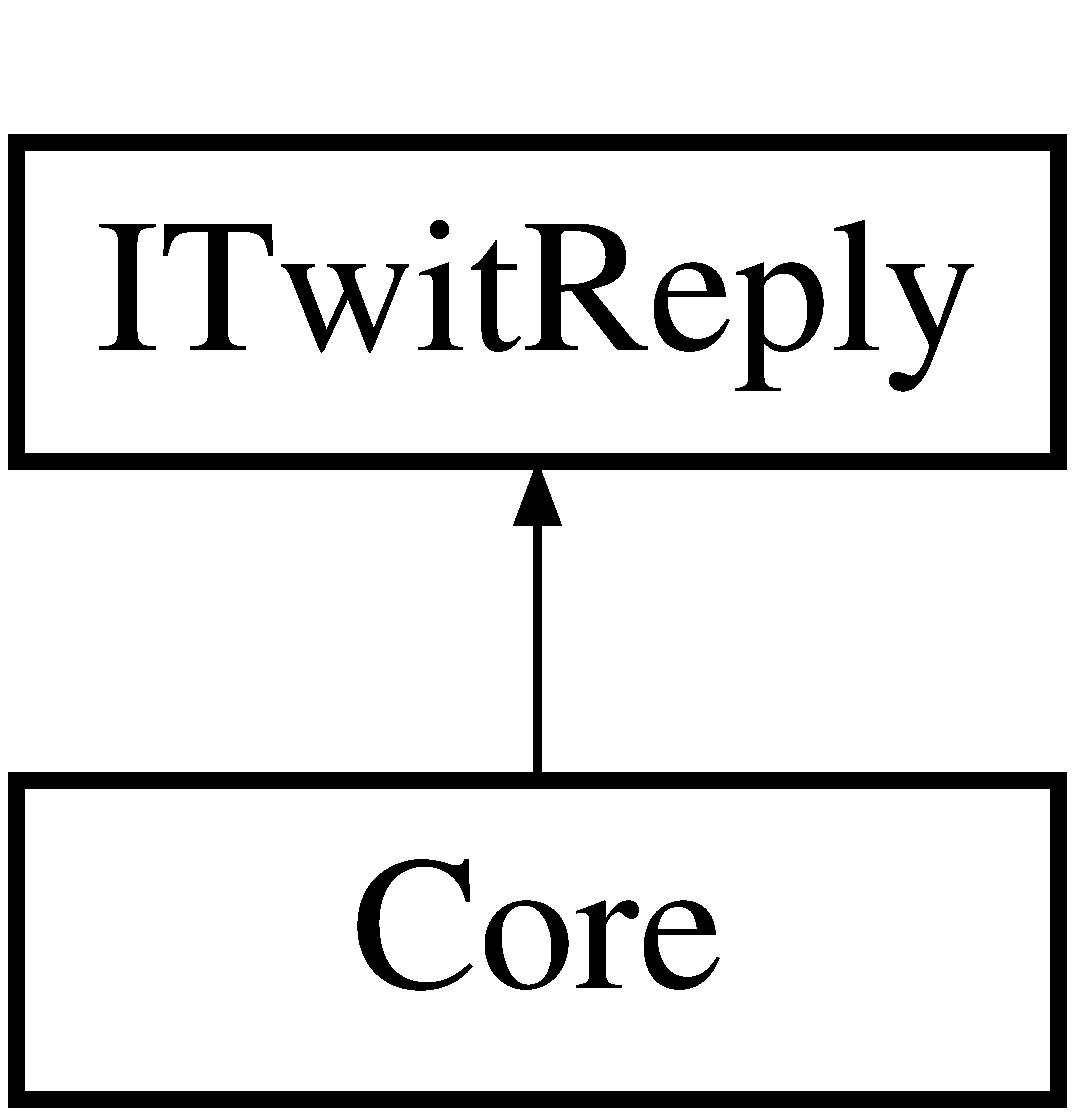
\includegraphics[height=2cm]{classCore}
\end{center}
\end{figure}
\subsection*{Public Slots}
\begin{CompactItemize}
\item 
void \hyperlink{classCore_2e3b63ac22f8fef5f2d2d5e9adc42cdd}{RequestStarted} (int id)
\item 
void \hyperlink{classCore_7b649f8d3aeae37e3f2e0eff65ab189f}{ReqFinished} (int id, bool error)
\item 
void \hyperlink{classCore_77844f4e1b5e81ff4a13bc22328a4258}{DataReadProgress} (int done, int total)
\item 
void \hyperlink{classCore_299d2e5e288da339e11f30500f473b16}{Done} (bool error)
\end{CompactItemize}
\subsection*{Signals}
\begin{CompactItemize}
\item 
void \hyperlink{classCore_c74c19f85f549851d3d7afd7e449770b}{QueryDone} ()
\end{CompactItemize}
\subsection*{Public Member Functions}
\begin{CompactItemize}
\item 
\hyperlink{classCore_4d99e39664e6f9a1b885742f92d83ade}{Core} (\hyperlink{classITwitReply}{ITwitReply} $\ast$obj)
\item 
virtual \hyperlink{classCore_776f8c46504b14183883c6273f93eaed}{$\sim$Core} ()
\item 
void \hyperlink{classCore_e07b32f495c64e768eb74cf50585352c}{GetPublicTimeline} ()
\item 
void \hyperlink{classCore_88d775139d0168f3fa24b4b4fda83386}{GetSingleStatus} (QString id)
\item 
void \hyperlink{classCore_c5f77029d34a1427c6b8a491c646e80b}{GetFeaturedUsers} ()
\item 
void \hyperlink{classCore_e4ec033e04b6490ac08d6f07507bc9c2}{Logout} ()
\item 
void \hyperlink{classCore_4570f9ad07c0ba58ce6326eb76568bf6}{Login} (QString user, QString passw)
\item 
void \hyperlink{classCore_7ba2a526280dcfc427480956f90f29cb}{GetDowntimeSchedule} ()
\item 
void \hyperlink{classCore_eeaa4a9429ac0a0dd2c2d11c0c0eea81}{IsTwitterUp} ()
\item 
void \hyperlink{classCore_7308eb02f04bd6da071db62f291c9def}{GetUsersTimeline} (\hyperlink{structSERVER_1_1Option2}{SERVER::Option2} $\ast$opt=NULL)
\item 
void \hyperlink{classCore_a896aea28b564e4841df4cf527fb0247}{GetFavorites} (QString user=\char`\"{}\char`\"{}, int page=1)
\item 
void \hyperlink{classCore_bc64aa3de63d39a878db543d8d5df9f5}{GetFriendsTimeline} (\hyperlink{structSERVER_1_1Option1}{SERVER::Option1} $\ast$opt=NULL)
\item 
void \hyperlink{classCore_7023af805b629e90a7aa2978366ee344}{PostNewStatus} (QString status)
\item 
void \hyperlink{classCore_b95dc3fca63c84496f6a487d845e7ba9}{GetRecentReplies} (\hyperlink{structSERVER_1_1Option3}{SERVER::Option3} $\ast$opt=NULL)
\item 
void \hyperlink{classCore_d881d4987b2845589443f74fb81da766}{RemoveStatus} (QString id)
\item 
void \hyperlink{classCore_2d41bfdcb5a2dff232ee299e83a7c8e6}{GetFriends} (\hyperlink{structSERVER_1_1Option4}{SERVER::Option4} $\ast$opt=NULL)
\item 
void \hyperlink{classCore_635c5c7bb0b6d2c2c6250ac050b466d6}{GetFollowers} (\hyperlink{structSERVER_1_1Option5}{SERVER::Option5} $\ast$opt=NULL)
\item 
void \hyperlink{classCore_572cef51b68ea351bdda246b5070c399}{GetUserDetails} (QString user)
\item 
void \hyperlink{classCore_1b43e65adc3ba72ae2bb344bec27eb53}{GetSentDirectMessages} (\hyperlink{structSERVER_1_1Option6}{SERVER::Option6} $\ast$opt=NULL)
\item 
void \hyperlink{classCore_5496ee42ce9d32aa0f98a2d56e3bbddf}{GetReceivedDirectMessages} (\hyperlink{structSERVER_1_1Option6}{SERVER::Option6} $\ast$opt=NULL)
\item 
void \hyperlink{classCore_f6afb71b9114a90e9b9856f64a6fe9cf}{SendDirectMessage} (QString user, QString text)
\item 
void \hyperlink{classCore_d98d496c44ebff775698737f8edbde44}{RemoveDirectMessage} (QString id)
\item 
void \hyperlink{classCore_3df3b62fa5366492a3eb4bba99f1849a}{AddFriendship} (QString user)
\item 
void \hyperlink{classCore_95ce85046d01f3d5d6928f06e8aab99c}{RemoveFriendship} (QString user)
\item 
void \hyperlink{classCore_0430da6765198a4f763ea7528f8e1e86}{FriendshipExist} (QString user\_\-a, QString user\_\-b)
\item 
void \hyperlink{classCore_e7b7355b923afe51411e3c949679904d}{VerifyCredentials} ()
\item 
void \hyperlink{classCore_62635d6cffb1fbef9f5c650518f83c67}{UpdateLocation} (QString location)
\item 
void \hyperlink{classCore_291a15a3ec5ebadc314c991f74cde776}{UpdateDeliveryDevice} (\hyperlink{namespaceSERVER_354160f0b752453a760c63ec882c8c87}{SERVER::DEVICES} device)
\item 
void \hyperlink{classCore_0cf4c10e33b1158e651977210312ea13}{RemainingApiRequests} ()
\item 
void \hyperlink{classCore_dbeb18bcc46253950b7660582d2eb5f5}{AddFavorite} (QString id)
\item 
void \hyperlink{classCore_c12e1d495cfea0a38c4adb38f258d27c}{RemoveFavorite} (QString id)
\item 
void \hyperlink{classCore_5cd0ceaff4b8d19b40f9b2e00839a286}{StartFollow} (QString user)
\item 
void \hyperlink{classCore_9a55db5cfe7788972b20d6a6bdc91218}{StopFollow} (QString user)
\item 
void \hyperlink{classCore_e715888efd76cc27271e4050ebed4c0b}{BlockUser} (QString user)
\item 
void \hyperlink{classCore_abc783553ec1e543435b8dc06f64939f}{UnBlockUser} (QString user)
\end{CompactItemize}


\subsection{Detailed Description}


Definition at line 12 of file Core.h.

\subsection{Constructor \& Destructor Documentation}
\hypertarget{classCore_4d99e39664e6f9a1b885742f92d83ade}{
\index{Core@{Core}!Core@{Core}}
\index{Core@{Core}!Core@{Core}}
\subsubsection{\setlength{\rightskip}{0pt plus 5cm}Core::Core ({\bf ITwitReply} $\ast$ {\em obj})}}
\label{classCore_4d99e39664e6f9a1b885742f92d83ade}




Definition at line 43 of file Core.cpp.\hypertarget{classCore_776f8c46504b14183883c6273f93eaed}{
\index{Core@{Core}!$\sim$Core@{$\sim$Core}}
\index{$\sim$Core@{$\sim$Core}!Core@{Core}}
\subsubsection{\setlength{\rightskip}{0pt plus 5cm}Core::$\sim$Core ()\hspace{0.3cm}{\tt  \mbox{[}virtual\mbox{]}}}}
\label{classCore_776f8c46504b14183883c6273f93eaed}




Definition at line 53 of file Core.cpp.

\subsection{Member Function Documentation}
\hypertarget{classCore_e07b32f495c64e768eb74cf50585352c}{
\index{Core@{Core}!GetPublicTimeline@{GetPublicTimeline}}
\index{GetPublicTimeline@{GetPublicTimeline}!Core@{Core}}
\subsubsection{\setlength{\rightskip}{0pt plus 5cm}void Core::GetPublicTimeline ()}}
\label{classCore_e07b32f495c64e768eb74cf50585352c}




Definition at line 180 of file Core.cpp.\hypertarget{classCore_88d775139d0168f3fa24b4b4fda83386}{
\index{Core@{Core}!GetSingleStatus@{GetSingleStatus}}
\index{GetSingleStatus@{GetSingleStatus}!Core@{Core}}
\subsubsection{\setlength{\rightskip}{0pt plus 5cm}void Core::GetSingleStatus (QString {\em id})}}
\label{classCore_88d775139d0168f3fa24b4b4fda83386}




Definition at line 186 of file Core.cpp.\hypertarget{classCore_c5f77029d34a1427c6b8a491c646e80b}{
\index{Core@{Core}!GetFeaturedUsers@{GetFeaturedUsers}}
\index{GetFeaturedUsers@{GetFeaturedUsers}!Core@{Core}}
\subsubsection{\setlength{\rightskip}{0pt plus 5cm}void Core::GetFeaturedUsers ()}}
\label{classCore_c5f77029d34a1427c6b8a491c646e80b}




Definition at line 195 of file Core.cpp.\hypertarget{classCore_e4ec033e04b6490ac08d6f07507bc9c2}{
\index{Core@{Core}!Logout@{Logout}}
\index{Logout@{Logout}!Core@{Core}}
\subsubsection{\setlength{\rightskip}{0pt plus 5cm}void Core::Logout ()}}
\label{classCore_e4ec033e04b6490ac08d6f07507bc9c2}




Definition at line 201 of file Core.cpp.\hypertarget{classCore_4570f9ad07c0ba58ce6326eb76568bf6}{
\index{Core@{Core}!Login@{Login}}
\index{Login@{Login}!Core@{Core}}
\subsubsection{\setlength{\rightskip}{0pt plus 5cm}void Core::Login (QString {\em user}, \/  QString {\em passw})}}
\label{classCore_4570f9ad07c0ba58ce6326eb76568bf6}




Definition at line 207 of file Core.cpp.\hypertarget{classCore_7ba2a526280dcfc427480956f90f29cb}{
\index{Core@{Core}!GetDowntimeSchedule@{GetDowntimeSchedule}}
\index{GetDowntimeSchedule@{GetDowntimeSchedule}!Core@{Core}}
\subsubsection{\setlength{\rightskip}{0pt plus 5cm}void Core::GetDowntimeSchedule ()}}
\label{classCore_7ba2a526280dcfc427480956f90f29cb}




Definition at line 213 of file Core.cpp.\hypertarget{classCore_eeaa4a9429ac0a0dd2c2d11c0c0eea81}{
\index{Core@{Core}!IsTwitterUp@{IsTwitterUp}}
\index{IsTwitterUp@{IsTwitterUp}!Core@{Core}}
\subsubsection{\setlength{\rightskip}{0pt plus 5cm}void Core::IsTwitterUp ()}}
\label{classCore_eeaa4a9429ac0a0dd2c2d11c0c0eea81}




Definition at line 219 of file Core.cpp.\hypertarget{classCore_7308eb02f04bd6da071db62f291c9def}{
\index{Core@{Core}!GetUsersTimeline@{GetUsersTimeline}}
\index{GetUsersTimeline@{GetUsersTimeline}!Core@{Core}}
\subsubsection{\setlength{\rightskip}{0pt plus 5cm}void Core::GetUsersTimeline ({\bf SERVER::Option2} $\ast$ {\em opt} = {\tt NULL})}}
\label{classCore_7308eb02f04bd6da071db62f291c9def}




Definition at line 225 of file Core.cpp.\hypertarget{classCore_a896aea28b564e4841df4cf527fb0247}{
\index{Core@{Core}!GetFavorites@{GetFavorites}}
\index{GetFavorites@{GetFavorites}!Core@{Core}}
\subsubsection{\setlength{\rightskip}{0pt plus 5cm}void Core::GetFavorites (QString {\em user} = {\tt \char`\"{}\char`\"{}}, \/  int {\em page} = {\tt 1})}}
\label{classCore_a896aea28b564e4841df4cf527fb0247}




Definition at line 256 of file Core.cpp.\hypertarget{classCore_bc64aa3de63d39a878db543d8d5df9f5}{
\index{Core@{Core}!GetFriendsTimeline@{GetFriendsTimeline}}
\index{GetFriendsTimeline@{GetFriendsTimeline}!Core@{Core}}
\subsubsection{\setlength{\rightskip}{0pt plus 5cm}void Core::GetFriendsTimeline ({\bf SERVER::Option1} $\ast$ {\em opt} = {\tt NULL})}}
\label{classCore_bc64aa3de63d39a878db543d8d5df9f5}




Definition at line 271 of file Core.cpp.\hypertarget{classCore_7023af805b629e90a7aa2978366ee344}{
\index{Core@{Core}!PostNewStatus@{PostNewStatus}}
\index{PostNewStatus@{PostNewStatus}!Core@{Core}}
\subsubsection{\setlength{\rightskip}{0pt plus 5cm}void Core::PostNewStatus (QString {\em status})}}
\label{classCore_7023af805b629e90a7aa2978366ee344}




Definition at line 292 of file Core.cpp.\hypertarget{classCore_b95dc3fca63c84496f6a487d845e7ba9}{
\index{Core@{Core}!GetRecentReplies@{GetRecentReplies}}
\index{GetRecentReplies@{GetRecentReplies}!Core@{Core}}
\subsubsection{\setlength{\rightskip}{0pt plus 5cm}void Core::GetRecentReplies ({\bf SERVER::Option3} $\ast$ {\em opt} = {\tt NULL})}}
\label{classCore_b95dc3fca63c84496f6a487d845e7ba9}




Definition at line 304 of file Core.cpp.\hypertarget{classCore_d881d4987b2845589443f74fb81da766}{
\index{Core@{Core}!RemoveStatus@{RemoveStatus}}
\index{RemoveStatus@{RemoveStatus}!Core@{Core}}
\subsubsection{\setlength{\rightskip}{0pt plus 5cm}void Core::RemoveStatus (QString {\em id})}}
\label{classCore_d881d4987b2845589443f74fb81da766}




Definition at line 323 of file Core.cpp.\hypertarget{classCore_2d41bfdcb5a2dff232ee299e83a7c8e6}{
\index{Core@{Core}!GetFriends@{GetFriends}}
\index{GetFriends@{GetFriends}!Core@{Core}}
\subsubsection{\setlength{\rightskip}{0pt plus 5cm}void Core::GetFriends ({\bf SERVER::Option4} $\ast$ {\em opt} = {\tt NULL})}}
\label{classCore_2d41bfdcb5a2dff232ee299e83a7c8e6}




Definition at line 333 of file Core.cpp.\hypertarget{classCore_635c5c7bb0b6d2c2c6250ac050b466d6}{
\index{Core@{Core}!GetFollowers@{GetFollowers}}
\index{GetFollowers@{GetFollowers}!Core@{Core}}
\subsubsection{\setlength{\rightskip}{0pt plus 5cm}void Core::GetFollowers ({\bf SERVER::Option5} $\ast$ {\em opt} = {\tt NULL})}}
\label{classCore_635c5c7bb0b6d2c2c6250ac050b466d6}




Definition at line 362 of file Core.cpp.\hypertarget{classCore_572cef51b68ea351bdda246b5070c399}{
\index{Core@{Core}!GetUserDetails@{GetUserDetails}}
\index{GetUserDetails@{GetUserDetails}!Core@{Core}}
\subsubsection{\setlength{\rightskip}{0pt plus 5cm}void Core::GetUserDetails (QString {\em user})}}
\label{classCore_572cef51b68ea351bdda246b5070c399}




Definition at line 389 of file Core.cpp.\hypertarget{classCore_1b43e65adc3ba72ae2bb344bec27eb53}{
\index{Core@{Core}!GetSentDirectMessages@{GetSentDirectMessages}}
\index{GetSentDirectMessages@{GetSentDirectMessages}!Core@{Core}}
\subsubsection{\setlength{\rightskip}{0pt plus 5cm}void Core::GetSentDirectMessages ({\bf SERVER::Option6} $\ast$ {\em opt} = {\tt NULL})}}
\label{classCore_1b43e65adc3ba72ae2bb344bec27eb53}




Definition at line 399 of file Core.cpp.\hypertarget{classCore_5496ee42ce9d32aa0f98a2d56e3bbddf}{
\index{Core@{Core}!GetReceivedDirectMessages@{GetReceivedDirectMessages}}
\index{GetReceivedDirectMessages@{GetReceivedDirectMessages}!Core@{Core}}
\subsubsection{\setlength{\rightskip}{0pt plus 5cm}void Core::GetReceivedDirectMessages ({\bf SERVER::Option6} $\ast$ {\em opt} = {\tt NULL})}}
\label{classCore_5496ee42ce9d32aa0f98a2d56e3bbddf}




Definition at line 418 of file Core.cpp.\hypertarget{classCore_f6afb71b9114a90e9b9856f64a6fe9cf}{
\index{Core@{Core}!SendDirectMessage@{SendDirectMessage}}
\index{SendDirectMessage@{SendDirectMessage}!Core@{Core}}
\subsubsection{\setlength{\rightskip}{0pt plus 5cm}void Core::SendDirectMessage (QString {\em user}, \/  QString {\em text})}}
\label{classCore_f6afb71b9114a90e9b9856f64a6fe9cf}




Definition at line 437 of file Core.cpp.\hypertarget{classCore_d98d496c44ebff775698737f8edbde44}{
\index{Core@{Core}!RemoveDirectMessage@{RemoveDirectMessage}}
\index{RemoveDirectMessage@{RemoveDirectMessage}!Core@{Core}}
\subsubsection{\setlength{\rightskip}{0pt plus 5cm}void Core::RemoveDirectMessage (QString {\em id})}}
\label{classCore_d98d496c44ebff775698737f8edbde44}




Definition at line 452 of file Core.cpp.\hypertarget{classCore_3df3b62fa5366492a3eb4bba99f1849a}{
\index{Core@{Core}!AddFriendship@{AddFriendship}}
\index{AddFriendship@{AddFriendship}!Core@{Core}}
\subsubsection{\setlength{\rightskip}{0pt plus 5cm}void Core::AddFriendship (QString {\em user})}}
\label{classCore_3df3b62fa5366492a3eb4bba99f1849a}




Definition at line 462 of file Core.cpp.\hypertarget{classCore_95ce85046d01f3d5d6928f06e8aab99c}{
\index{Core@{Core}!RemoveFriendship@{RemoveFriendship}}
\index{RemoveFriendship@{RemoveFriendship}!Core@{Core}}
\subsubsection{\setlength{\rightskip}{0pt plus 5cm}void Core::RemoveFriendship (QString {\em user})}}
\label{classCore_95ce85046d01f3d5d6928f06e8aab99c}




Definition at line 472 of file Core.cpp.\hypertarget{classCore_0430da6765198a4f763ea7528f8e1e86}{
\index{Core@{Core}!FriendshipExist@{FriendshipExist}}
\index{FriendshipExist@{FriendshipExist}!Core@{Core}}
\subsubsection{\setlength{\rightskip}{0pt plus 5cm}void Core::FriendshipExist (QString {\em user\_\-a}, \/  QString {\em user\_\-b})}}
\label{classCore_0430da6765198a4f763ea7528f8e1e86}




Definition at line 482 of file Core.cpp.\hypertarget{classCore_e7b7355b923afe51411e3c949679904d}{
\index{Core@{Core}!VerifyCredentials@{VerifyCredentials}}
\index{VerifyCredentials@{VerifyCredentials}!Core@{Core}}
\subsubsection{\setlength{\rightskip}{0pt plus 5cm}void Core::VerifyCredentials ()}}
\label{classCore_e7b7355b923afe51411e3c949679904d}




Definition at line 493 of file Core.cpp.\hypertarget{classCore_62635d6cffb1fbef9f5c650518f83c67}{
\index{Core@{Core}!UpdateLocation@{UpdateLocation}}
\index{UpdateLocation@{UpdateLocation}!Core@{Core}}
\subsubsection{\setlength{\rightskip}{0pt plus 5cm}void Core::UpdateLocation (QString {\em location})}}
\label{classCore_62635d6cffb1fbef9f5c650518f83c67}




Definition at line 499 of file Core.cpp.\hypertarget{classCore_291a15a3ec5ebadc314c991f74cde776}{
\index{Core@{Core}!UpdateDeliveryDevice@{UpdateDeliveryDevice}}
\index{UpdateDeliveryDevice@{UpdateDeliveryDevice}!Core@{Core}}
\subsubsection{\setlength{\rightskip}{0pt plus 5cm}void Core::UpdateDeliveryDevice ({\bf SERVER::DEVICES} {\em device})}}
\label{classCore_291a15a3ec5ebadc314c991f74cde776}




Definition at line 511 of file Core.cpp.\hypertarget{classCore_0cf4c10e33b1158e651977210312ea13}{
\index{Core@{Core}!RemainingApiRequests@{RemainingApiRequests}}
\index{RemainingApiRequests@{RemainingApiRequests}!Core@{Core}}
\subsubsection{\setlength{\rightskip}{0pt plus 5cm}void Core::RemainingApiRequests ()}}
\label{classCore_0cf4c10e33b1158e651977210312ea13}




Definition at line 532 of file Core.cpp.\hypertarget{classCore_dbeb18bcc46253950b7660582d2eb5f5}{
\index{Core@{Core}!AddFavorite@{AddFavorite}}
\index{AddFavorite@{AddFavorite}!Core@{Core}}
\subsubsection{\setlength{\rightskip}{0pt plus 5cm}void Core::AddFavorite (QString {\em id})}}
\label{classCore_dbeb18bcc46253950b7660582d2eb5f5}




Definition at line 538 of file Core.cpp.\hypertarget{classCore_c12e1d495cfea0a38c4adb38f258d27c}{
\index{Core@{Core}!RemoveFavorite@{RemoveFavorite}}
\index{RemoveFavorite@{RemoveFavorite}!Core@{Core}}
\subsubsection{\setlength{\rightskip}{0pt plus 5cm}void Core::RemoveFavorite (QString {\em id})}}
\label{classCore_c12e1d495cfea0a38c4adb38f258d27c}




Definition at line 548 of file Core.cpp.\hypertarget{classCore_5cd0ceaff4b8d19b40f9b2e00839a286}{
\index{Core@{Core}!StartFollow@{StartFollow}}
\index{StartFollow@{StartFollow}!Core@{Core}}
\subsubsection{\setlength{\rightskip}{0pt plus 5cm}void Core::StartFollow (QString {\em user})}}
\label{classCore_5cd0ceaff4b8d19b40f9b2e00839a286}




Definition at line 558 of file Core.cpp.\hypertarget{classCore_9a55db5cfe7788972b20d6a6bdc91218}{
\index{Core@{Core}!StopFollow@{StopFollow}}
\index{StopFollow@{StopFollow}!Core@{Core}}
\subsubsection{\setlength{\rightskip}{0pt plus 5cm}void Core::StopFollow (QString {\em user})}}
\label{classCore_9a55db5cfe7788972b20d6a6bdc91218}




Definition at line 568 of file Core.cpp.\hypertarget{classCore_e715888efd76cc27271e4050ebed4c0b}{
\index{Core@{Core}!BlockUser@{BlockUser}}
\index{BlockUser@{BlockUser}!Core@{Core}}
\subsubsection{\setlength{\rightskip}{0pt plus 5cm}void Core::BlockUser (QString {\em user})}}
\label{classCore_e715888efd76cc27271e4050ebed4c0b}




Definition at line 578 of file Core.cpp.\hypertarget{classCore_abc783553ec1e543435b8dc06f64939f}{
\index{Core@{Core}!UnBlockUser@{UnBlockUser}}
\index{UnBlockUser@{UnBlockUser}!Core@{Core}}
\subsubsection{\setlength{\rightskip}{0pt plus 5cm}void Core::UnBlockUser (QString {\em user})}}
\label{classCore_abc783553ec1e543435b8dc06f64939f}




Definition at line 588 of file Core.cpp.\hypertarget{classCore_2e3b63ac22f8fef5f2d2d5e9adc42cdd}{
\index{Core@{Core}!RequestStarted@{RequestStarted}}
\index{RequestStarted@{RequestStarted}!Core@{Core}}
\subsubsection{\setlength{\rightskip}{0pt plus 5cm}void Core::RequestStarted (int {\em id})\hspace{0.3cm}{\tt  \mbox{[}slot\mbox{]}}}}
\label{classCore_2e3b63ac22f8fef5f2d2d5e9adc42cdd}




Definition at line 98 of file Core.cpp.\hypertarget{classCore_7b649f8d3aeae37e3f2e0eff65ab189f}{
\index{Core@{Core}!ReqFinished@{ReqFinished}}
\index{ReqFinished@{ReqFinished}!Core@{Core}}
\subsubsection{\setlength{\rightskip}{0pt plus 5cm}void Core::ReqFinished (int {\em id}, \/  bool {\em error})\hspace{0.3cm}{\tt  \mbox{[}slot\mbox{]}}}}
\label{classCore_7b649f8d3aeae37e3f2e0eff65ab189f}




Definition at line 101 of file Core.cpp.\hypertarget{classCore_77844f4e1b5e81ff4a13bc22328a4258}{
\index{Core@{Core}!DataReadProgress@{DataReadProgress}}
\index{DataReadProgress@{DataReadProgress}!Core@{Core}}
\subsubsection{\setlength{\rightskip}{0pt plus 5cm}void Core::DataReadProgress (int {\em done}, \/  int {\em total})\hspace{0.3cm}{\tt  \mbox{[}slot\mbox{]}}}}
\label{classCore_77844f4e1b5e81ff4a13bc22328a4258}




Definition at line 75 of file Core.cpp.\hypertarget{classCore_299d2e5e288da339e11f30500f473b16}{
\index{Core@{Core}!Done@{Done}}
\index{Done@{Done}!Core@{Core}}
\subsubsection{\setlength{\rightskip}{0pt plus 5cm}void Core::Done (bool {\em error})\hspace{0.3cm}{\tt  \mbox{[}slot\mbox{]}}}}
\label{classCore_299d2e5e288da339e11f30500f473b16}




Definition at line 70 of file Core.cpp.\hypertarget{classCore_c74c19f85f549851d3d7afd7e449770b}{
\index{Core@{Core}!QueryDone@{QueryDone}}
\index{QueryDone@{QueryDone}!Core@{Core}}
\subsubsection{\setlength{\rightskip}{0pt plus 5cm}void Core::QueryDone ()\hspace{0.3cm}{\tt  \mbox{[}signal\mbox{]}}}}
\label{classCore_c74c19f85f549851d3d7afd7e449770b}




Definition at line 88 of file moc\_\-Core.cpp.

The documentation for this class was generated from the following files:\begin{CompactItemize}
\item 
include/\hyperlink{Core_8h}{Core.h}\item 
generated/\hyperlink{moc__Core_8cpp}{moc\_\-Core.cpp}\item 
src/\hyperlink{Core_8cpp}{Core.cpp}\end{CompactItemize}

\hypertarget{classITwitReply}{
\section{ITwitReply Class Reference}
\label{classITwitReply}\index{ITwitReply@{ITwitReply}}
}
{\tt \#include $<$ITwitReply.h$>$}

Inheritance diagram for ITwitReply::\begin{figure}[H]
\begin{center}
\leavevmode
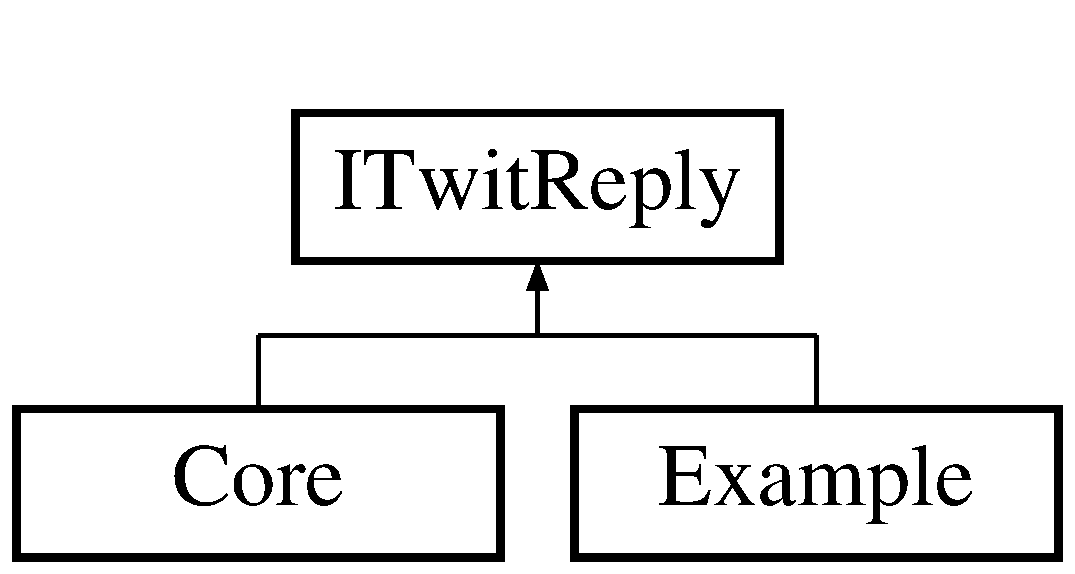
\includegraphics[height=2cm]{classITwitReply}
\end{center}
\end{figure}
\subsection*{Public Member Functions}
\begin{CompactItemize}
\item 
virtual void \hyperlink{classITwitReply_9cc4c9da62c570e6e076f2a7ce52b75a}{OnError} (std::string error)=0
\item 
virtual void \hyperlink{classITwitReply_a103f872024b0a36e669b0d82a26a528}{OnMessageReceived} (std::string message)=0
\item 
virtual void \hyperlink{classITwitReply_9011b418bb62f734a2e3cd447815ec90}{OnStatusReceived} (\hyperlink{namespaceSERVER_e274de6af58152c34520420007dfa0ea}{SERVER::RESP} response)=0
\item 
virtual void \hyperlink{classITwitReply_691e9bcbe06bd66233b1c870d2e4d67d}{OnLoginStatus} (bool isLoggedIn)=0
\end{CompactItemize}


\subsection{Detailed Description}


Definition at line 6 of file ITwitReply.h.

\subsection{Member Function Documentation}
\hypertarget{classITwitReply_9cc4c9da62c570e6e076f2a7ce52b75a}{
\index{ITwitReply@{ITwitReply}!OnError@{OnError}}
\index{OnError@{OnError}!ITwitReply@{ITwitReply}}
\subsubsection{\setlength{\rightskip}{0pt plus 5cm}virtual void ITwitReply::OnError (std::string {\em error})\hspace{0.3cm}{\tt  \mbox{[}pure virtual\mbox{]}}}}
\label{classITwitReply_9cc4c9da62c570e6e076f2a7ce52b75a}


\hypertarget{classITwitReply_a103f872024b0a36e669b0d82a26a528}{
\index{ITwitReply@{ITwitReply}!OnMessageReceived@{OnMessageReceived}}
\index{OnMessageReceived@{OnMessageReceived}!ITwitReply@{ITwitReply}}
\subsubsection{\setlength{\rightskip}{0pt plus 5cm}virtual void ITwitReply::OnMessageReceived (std::string {\em message})\hspace{0.3cm}{\tt  \mbox{[}pure virtual\mbox{]}}}}
\label{classITwitReply_a103f872024b0a36e669b0d82a26a528}


\hypertarget{classITwitReply_9011b418bb62f734a2e3cd447815ec90}{
\index{ITwitReply@{ITwitReply}!OnStatusReceived@{OnStatusReceived}}
\index{OnStatusReceived@{OnStatusReceived}!ITwitReply@{ITwitReply}}
\subsubsection{\setlength{\rightskip}{0pt plus 5cm}virtual void ITwitReply::OnStatusReceived ({\bf SERVER::RESP} {\em response})\hspace{0.3cm}{\tt  \mbox{[}pure virtual\mbox{]}}}}
\label{classITwitReply_9011b418bb62f734a2e3cd447815ec90}


\hypertarget{classITwitReply_691e9bcbe06bd66233b1c870d2e4d67d}{
\index{ITwitReply@{ITwitReply}!OnLoginStatus@{OnLoginStatus}}
\index{OnLoginStatus@{OnLoginStatus}!ITwitReply@{ITwitReply}}
\subsubsection{\setlength{\rightskip}{0pt plus 5cm}virtual void ITwitReply::OnLoginStatus (bool {\em isLoggedIn})\hspace{0.3cm}{\tt  \mbox{[}pure virtual\mbox{]}}}}
\label{classITwitReply_691e9bcbe06bd66233b1c870d2e4d67d}




The documentation for this class was generated from the following file:\begin{CompactItemize}
\item 
include/\hyperlink{ITwitReply_8h}{ITwitReply.h}\end{CompactItemize}

\hypertarget{structSERVER_1_1Option1}{
\section{SERVER::Option1 Struct Reference}
\label{structSERVER_1_1Option1}\index{SERVER::Option1@{SERVER::Option1}}
}
{\tt \#include $<$Server.h$>$}

\subsection*{Public Member Functions}
\begin{CompactItemize}
\item 
\hyperlink{structSERVER_1_1Option1_f5c6a93cd6119cec081dab70fcb342d6}{Option1} ()
\end{CompactItemize}
\subsection*{Public Attributes}
\begin{CompactItemize}
\item 
std::string \hyperlink{structSERVER_1_1Option1_ab0f16c33d1a47822ab2622f1a8e03b4}{since}
\begin{CompactList}\small\item\em Optional. Narrows the returned results to just those statuses created after the specified HTTP-formatted date. \item\end{CompactList}\item 
int \hyperlink{structSERVER_1_1Option1_30def1c303684fd431b3cb2d78fbe18d}{sinceId}
\begin{CompactList}\small\item\em Optional. Returns only statuses with an ID greater than (that is, more recent than) the specified ID. \item\end{CompactList}\item 
int \hyperlink{structSERVER_1_1Option1_20b51548aa06990c9e1f5b5fd8d878e5}{count}
\begin{CompactList}\small\item\em Optional. Specifies the number of statuses to retrieve. May not be greater than 200. \item\end{CompactList}\item 
int \hyperlink{structSERVER_1_1Option1_00eb077ba9bbe459a38aea89f1c71426}{page}
\begin{CompactList}\small\item\em Optional. Specify which page to return. \item\end{CompactList}\end{CompactItemize}


\subsection{Detailed Description}


Definition at line 22 of file Server.h.

\subsection{Constructor \& Destructor Documentation}
\hypertarget{structSERVER_1_1Option1_f5c6a93cd6119cec081dab70fcb342d6}{
\index{SERVER::Option1@{SERVER::Option1}!Option1@{Option1}}
\index{Option1@{Option1}!SERVER::Option1@{SERVER::Option1}}
\subsubsection{\setlength{\rightskip}{0pt plus 5cm}SERVER::Option1::Option1 ()\hspace{0.3cm}{\tt  \mbox{[}inline\mbox{]}}}}
\label{structSERVER_1_1Option1_f5c6a93cd6119cec081dab70fcb342d6}




Definition at line 24 of file Server.h.

\subsection{Member Data Documentation}
\hypertarget{structSERVER_1_1Option1_ab0f16c33d1a47822ab2622f1a8e03b4}{
\index{SERVER::Option1@{SERVER::Option1}!since@{since}}
\index{since@{since}!SERVER::Option1@{SERVER::Option1}}
\subsubsection{\setlength{\rightskip}{0pt plus 5cm}std::string {\bf SERVER::Option1::since}}}
\label{structSERVER_1_1Option1_ab0f16c33d1a47822ab2622f1a8e03b4}


Optional. Narrows the returned results to just those statuses created after the specified HTTP-formatted date. 



Definition at line 26 of file Server.h.\hypertarget{structSERVER_1_1Option1_30def1c303684fd431b3cb2d78fbe18d}{
\index{SERVER::Option1@{SERVER::Option1}!sinceId@{sinceId}}
\index{sinceId@{sinceId}!SERVER::Option1@{SERVER::Option1}}
\subsubsection{\setlength{\rightskip}{0pt plus 5cm}int {\bf SERVER::Option1::sinceId}}}
\label{structSERVER_1_1Option1_30def1c303684fd431b3cb2d78fbe18d}


Optional. Returns only statuses with an ID greater than (that is, more recent than) the specified ID. 



Definition at line 28 of file Server.h.\hypertarget{structSERVER_1_1Option1_20b51548aa06990c9e1f5b5fd8d878e5}{
\index{SERVER::Option1@{SERVER::Option1}!count@{count}}
\index{count@{count}!SERVER::Option1@{SERVER::Option1}}
\subsubsection{\setlength{\rightskip}{0pt plus 5cm}int {\bf SERVER::Option1::count}}}
\label{structSERVER_1_1Option1_20b51548aa06990c9e1f5b5fd8d878e5}


Optional. Specifies the number of statuses to retrieve. May not be greater than 200. 



Definition at line 30 of file Server.h.\hypertarget{structSERVER_1_1Option1_00eb077ba9bbe459a38aea89f1c71426}{
\index{SERVER::Option1@{SERVER::Option1}!page@{page}}
\index{page@{page}!SERVER::Option1@{SERVER::Option1}}
\subsubsection{\setlength{\rightskip}{0pt plus 5cm}int {\bf SERVER::Option1::page}}}
\label{structSERVER_1_1Option1_00eb077ba9bbe459a38aea89f1c71426}


Optional. Specify which page to return. 



Definition at line 32 of file Server.h.

The documentation for this struct was generated from the following file:\begin{CompactItemize}
\item 
include/\hyperlink{Server_8h}{Server.h}\end{CompactItemize}

\hypertarget{structSERVER_1_1Option2}{
\section{SERVER::Option2 Struct Reference}
\label{structSERVER_1_1Option2}\index{SERVER::Option2@{SERVER::Option2}}
}
{\tt \#include $<$Server.h$>$}

\subsection*{Public Member Functions}
\begin{CompactItemize}
\item 
\hyperlink{structSERVER_1_1Option2_d97991e3af57fa03d4763ff00fee831c}{Option2} ()
\end{CompactItemize}
\subsection*{Public Attributes}
\begin{CompactItemize}
\item 
std::string \hyperlink{structSERVER_1_1Option2_cc4ff418bf1cb85987457878ecf58840}{user}
\begin{CompactList}\small\item\em Optional. Specifies the ID or screen name of the user for whom to return the friends\_\-timeline. \item\end{CompactList}\item 
int \hyperlink{structSERVER_1_1Option2_49cccf8e4da75bacccc85eb3ea4257e7}{count}
\begin{CompactList}\small\item\em Optional. Specifies the number of statuses to retrieve. May not be greater than 200. \item\end{CompactList}\item 
std::string \hyperlink{structSERVER_1_1Option2_a5f812a1c4b4a757204e187a90a99d92}{since}
\begin{CompactList}\small\item\em Optional. Narrows the returned results to just those statuses created after the specified HTTP-formatted date. \item\end{CompactList}\item 
int \hyperlink{structSERVER_1_1Option2_42cf95d44c8dee885c20570746b52cfa}{sinceId}
\begin{CompactList}\small\item\em Optional. Returns only statuses with an ID greater than (that is, more recent than) the specified ID. \item\end{CompactList}\item 
int \hyperlink{structSERVER_1_1Option2_e5527a71b27b55dfbf1dc2a0847a1b98}{page}
\begin{CompactList}\small\item\em Optional. Specify which page to return. \item\end{CompactList}\end{CompactItemize}


\subsection{Detailed Description}


Definition at line 35 of file Server.h.

\subsection{Constructor \& Destructor Documentation}
\hypertarget{structSERVER_1_1Option2_d97991e3af57fa03d4763ff00fee831c}{
\index{SERVER::Option2@{SERVER::Option2}!Option2@{Option2}}
\index{Option2@{Option2}!SERVER::Option2@{SERVER::Option2}}
\subsubsection{\setlength{\rightskip}{0pt plus 5cm}SERVER::Option2::Option2 ()\hspace{0.3cm}{\tt  \mbox{[}inline\mbox{]}}}}
\label{structSERVER_1_1Option2_d97991e3af57fa03d4763ff00fee831c}




Definition at line 37 of file Server.h.

\subsection{Member Data Documentation}
\hypertarget{structSERVER_1_1Option2_cc4ff418bf1cb85987457878ecf58840}{
\index{SERVER::Option2@{SERVER::Option2}!user@{user}}
\index{user@{user}!SERVER::Option2@{SERVER::Option2}}
\subsubsection{\setlength{\rightskip}{0pt plus 5cm}std::string {\bf SERVER::Option2::user}}}
\label{structSERVER_1_1Option2_cc4ff418bf1cb85987457878ecf58840}


Optional. Specifies the ID or screen name of the user for whom to return the friends\_\-timeline. 



Definition at line 39 of file Server.h.\hypertarget{structSERVER_1_1Option2_49cccf8e4da75bacccc85eb3ea4257e7}{
\index{SERVER::Option2@{SERVER::Option2}!count@{count}}
\index{count@{count}!SERVER::Option2@{SERVER::Option2}}
\subsubsection{\setlength{\rightskip}{0pt plus 5cm}int {\bf SERVER::Option2::count}}}
\label{structSERVER_1_1Option2_49cccf8e4da75bacccc85eb3ea4257e7}


Optional. Specifies the number of statuses to retrieve. May not be greater than 200. 



Definition at line 41 of file Server.h.\hypertarget{structSERVER_1_1Option2_a5f812a1c4b4a757204e187a90a99d92}{
\index{SERVER::Option2@{SERVER::Option2}!since@{since}}
\index{since@{since}!SERVER::Option2@{SERVER::Option2}}
\subsubsection{\setlength{\rightskip}{0pt plus 5cm}std::string {\bf SERVER::Option2::since}}}
\label{structSERVER_1_1Option2_a5f812a1c4b4a757204e187a90a99d92}


Optional. Narrows the returned results to just those statuses created after the specified HTTP-formatted date. 



Definition at line 43 of file Server.h.\hypertarget{structSERVER_1_1Option2_42cf95d44c8dee885c20570746b52cfa}{
\index{SERVER::Option2@{SERVER::Option2}!sinceId@{sinceId}}
\index{sinceId@{sinceId}!SERVER::Option2@{SERVER::Option2}}
\subsubsection{\setlength{\rightskip}{0pt plus 5cm}int {\bf SERVER::Option2::sinceId}}}
\label{structSERVER_1_1Option2_42cf95d44c8dee885c20570746b52cfa}


Optional. Returns only statuses with an ID greater than (that is, more recent than) the specified ID. 



Definition at line 45 of file Server.h.\hypertarget{structSERVER_1_1Option2_e5527a71b27b55dfbf1dc2a0847a1b98}{
\index{SERVER::Option2@{SERVER::Option2}!page@{page}}
\index{page@{page}!SERVER::Option2@{SERVER::Option2}}
\subsubsection{\setlength{\rightskip}{0pt plus 5cm}int {\bf SERVER::Option2::page}}}
\label{structSERVER_1_1Option2_e5527a71b27b55dfbf1dc2a0847a1b98}


Optional. Specify which page to return. 



Definition at line 47 of file Server.h.

The documentation for this struct was generated from the following file:\begin{CompactItemize}
\item 
include/\hyperlink{Server_8h}{Server.h}\end{CompactItemize}

\hypertarget{structSERVER_1_1Option3}{
\section{SERVER::Option3 Struct Reference}
\label{structSERVER_1_1Option3}\index{SERVER::Option3@{SERVER::Option3}}
}
{\tt \#include $<$Server.h$>$}

\subsection*{Public Member Functions}
\begin{CompactItemize}
\item 
\hyperlink{structSERVER_1_1Option3_aa0c40ea1bb475515e5e810c05ce4dca}{Option3} ()
\end{CompactItemize}
\subsection*{Public Attributes}
\begin{CompactItemize}
\item 
int \hyperlink{structSERVER_1_1Option3_94f1d27b09f86c44d18275a3c3f2697d}{page}
\begin{CompactList}\small\item\em Optional. Specify which page to return. \item\end{CompactList}\item 
std::string \hyperlink{structSERVER_1_1Option3_f2d56b690d7b755c4ca88869dfcf9ff6}{since}
\begin{CompactList}\small\item\em Optional. Narrows the returned results to just those statuses created after the specified HTTP-formatted date. \item\end{CompactList}\item 
int \hyperlink{structSERVER_1_1Option3_7acbe4cffada84ed124186614322c162}{sinceId}
\begin{CompactList}\small\item\em Optional. Returns only statuses with an ID greater than (that is, more recent than) the specified ID. \item\end{CompactList}\end{CompactItemize}


\subsection{Detailed Description}


Definition at line 50 of file Server.h.

\subsection{Constructor \& Destructor Documentation}
\hypertarget{structSERVER_1_1Option3_aa0c40ea1bb475515e5e810c05ce4dca}{
\index{SERVER::Option3@{SERVER::Option3}!Option3@{Option3}}
\index{Option3@{Option3}!SERVER::Option3@{SERVER::Option3}}
\subsubsection{\setlength{\rightskip}{0pt plus 5cm}SERVER::Option3::Option3 ()\hspace{0.3cm}{\tt  \mbox{[}inline\mbox{]}}}}
\label{structSERVER_1_1Option3_aa0c40ea1bb475515e5e810c05ce4dca}




Definition at line 52 of file Server.h.

\subsection{Member Data Documentation}
\hypertarget{structSERVER_1_1Option3_94f1d27b09f86c44d18275a3c3f2697d}{
\index{SERVER::Option3@{SERVER::Option3}!page@{page}}
\index{page@{page}!SERVER::Option3@{SERVER::Option3}}
\subsubsection{\setlength{\rightskip}{0pt plus 5cm}int {\bf SERVER::Option3::page}}}
\label{structSERVER_1_1Option3_94f1d27b09f86c44d18275a3c3f2697d}


Optional. Specify which page to return. 



Definition at line 54 of file Server.h.\hypertarget{structSERVER_1_1Option3_f2d56b690d7b755c4ca88869dfcf9ff6}{
\index{SERVER::Option3@{SERVER::Option3}!since@{since}}
\index{since@{since}!SERVER::Option3@{SERVER::Option3}}
\subsubsection{\setlength{\rightskip}{0pt plus 5cm}std::string {\bf SERVER::Option3::since}}}
\label{structSERVER_1_1Option3_f2d56b690d7b755c4ca88869dfcf9ff6}


Optional. Narrows the returned results to just those statuses created after the specified HTTP-formatted date. 



Definition at line 56 of file Server.h.\hypertarget{structSERVER_1_1Option3_7acbe4cffada84ed124186614322c162}{
\index{SERVER::Option3@{SERVER::Option3}!sinceId@{sinceId}}
\index{sinceId@{sinceId}!SERVER::Option3@{SERVER::Option3}}
\subsubsection{\setlength{\rightskip}{0pt plus 5cm}int {\bf SERVER::Option3::sinceId}}}
\label{structSERVER_1_1Option3_7acbe4cffada84ed124186614322c162}


Optional. Returns only statuses with an ID greater than (that is, more recent than) the specified ID. 



Definition at line 58 of file Server.h.

The documentation for this struct was generated from the following file:\begin{CompactItemize}
\item 
include/\hyperlink{Server_8h}{Server.h}\end{CompactItemize}

\hypertarget{structSERVER_1_1Option4}{
\section{SERVER::Option4 Struct Reference}
\label{structSERVER_1_1Option4}\index{SERVER::Option4@{SERVER::Option4}}
}
{\tt \#include $<$Server.h$>$}

\subsection*{Public Member Functions}
\begin{CompactItemize}
\item 
\hyperlink{structSERVER_1_1Option4_b641f3c3122d862af9d365ff219f7219}{Option4} ()
\end{CompactItemize}
\subsection*{Public Attributes}
\begin{CompactItemize}
\item 
std::string \hyperlink{structSERVER_1_1Option4_3ba9825ad8182388e55c978bf9b1867f}{user}
\begin{CompactList}\small\item\em Optional. The ID or screen name of the user for whom to request a list of friends. \item\end{CompactList}\item 
int \hyperlink{structSERVER_1_1Option4_f93ca2adc6bbaef592b92364c492a97d}{page}
\begin{CompactList}\small\item\em Optional. Specify which page to return. \item\end{CompactList}\item 
bool \hyperlink{structSERVER_1_1Option4_d5cb29165acf0bef7d33e2b1bbd034a1}{lite}
\begin{CompactList}\small\item\em Optional. Prevents the inline inclusion of current status. Must be set to a value of true. \item\end{CompactList}\item 
std::string \hyperlink{structSERVER_1_1Option4_4d7eaf322b263a5a82cc9010e24def48}{since}
\begin{CompactList}\small\item\em Optional. Narrows the returned results to just those statuses created after the specified HTTP-formatted date. \item\end{CompactList}\end{CompactItemize}


\subsection{Detailed Description}


Definition at line 61 of file Server.h.

\subsection{Constructor \& Destructor Documentation}
\hypertarget{structSERVER_1_1Option4_b641f3c3122d862af9d365ff219f7219}{
\index{SERVER::Option4@{SERVER::Option4}!Option4@{Option4}}
\index{Option4@{Option4}!SERVER::Option4@{SERVER::Option4}}
\subsubsection{\setlength{\rightskip}{0pt plus 5cm}SERVER::Option4::Option4 ()\hspace{0.3cm}{\tt  \mbox{[}inline\mbox{]}}}}
\label{structSERVER_1_1Option4_b641f3c3122d862af9d365ff219f7219}




Definition at line 63 of file Server.h.

\subsection{Member Data Documentation}
\hypertarget{structSERVER_1_1Option4_3ba9825ad8182388e55c978bf9b1867f}{
\index{SERVER::Option4@{SERVER::Option4}!user@{user}}
\index{user@{user}!SERVER::Option4@{SERVER::Option4}}
\subsubsection{\setlength{\rightskip}{0pt plus 5cm}std::string {\bf SERVER::Option4::user}}}
\label{structSERVER_1_1Option4_3ba9825ad8182388e55c978bf9b1867f}


Optional. The ID or screen name of the user for whom to request a list of friends. 



Definition at line 65 of file Server.h.\hypertarget{structSERVER_1_1Option4_f93ca2adc6bbaef592b92364c492a97d}{
\index{SERVER::Option4@{SERVER::Option4}!page@{page}}
\index{page@{page}!SERVER::Option4@{SERVER::Option4}}
\subsubsection{\setlength{\rightskip}{0pt plus 5cm}int {\bf SERVER::Option4::page}}}
\label{structSERVER_1_1Option4_f93ca2adc6bbaef592b92364c492a97d}


Optional. Specify which page to return. 



Definition at line 67 of file Server.h.\hypertarget{structSERVER_1_1Option4_d5cb29165acf0bef7d33e2b1bbd034a1}{
\index{SERVER::Option4@{SERVER::Option4}!lite@{lite}}
\index{lite@{lite}!SERVER::Option4@{SERVER::Option4}}
\subsubsection{\setlength{\rightskip}{0pt plus 5cm}bool {\bf SERVER::Option4::lite}}}
\label{structSERVER_1_1Option4_d5cb29165acf0bef7d33e2b1bbd034a1}


Optional. Prevents the inline inclusion of current status. Must be set to a value of true. 



Definition at line 69 of file Server.h.\hypertarget{structSERVER_1_1Option4_4d7eaf322b263a5a82cc9010e24def48}{
\index{SERVER::Option4@{SERVER::Option4}!since@{since}}
\index{since@{since}!SERVER::Option4@{SERVER::Option4}}
\subsubsection{\setlength{\rightskip}{0pt plus 5cm}std::string {\bf SERVER::Option4::since}}}
\label{structSERVER_1_1Option4_4d7eaf322b263a5a82cc9010e24def48}


Optional. Narrows the returned results to just those statuses created after the specified HTTP-formatted date. 



Definition at line 71 of file Server.h.

The documentation for this struct was generated from the following file:\begin{CompactItemize}
\item 
include/\hyperlink{Server_8h}{Server.h}\end{CompactItemize}

\hypertarget{structSERVER_1_1Option5}{
\section{SERVER::Option5 Struct Reference}
\label{structSERVER_1_1Option5}\index{SERVER::Option5@{SERVER::Option5}}
}
{\tt \#include $<$Server.h$>$}

\subsection*{Public Member Functions}
\begin{CompactItemize}
\item 
\hyperlink{structSERVER_1_1Option5_7d84350b26df14847f34a16682d4e265}{Option5} ()
\end{CompactItemize}
\subsection*{Public Attributes}
\begin{CompactItemize}
\item 
std::string \hyperlink{structSERVER_1_1Option5_edba226344f8de6938f0ee804cb5fe10}{user}
\begin{CompactList}\small\item\em Optional. The ID or screen name of the user for whom to request a list of followers. \item\end{CompactList}\item 
int \hyperlink{structSERVER_1_1Option5_629b118bef583584f946c6acea5909e9}{page}
\begin{CompactList}\small\item\em Optional. Specify which page to return. \item\end{CompactList}\item 
bool \hyperlink{structSERVER_1_1Option5_18f4978757ae6b72d8007976964c7d71}{lite}
\begin{CompactList}\small\item\em Optional. Prevents the inline inclusion of current status. Must be set to a value of true. \item\end{CompactList}\end{CompactItemize}


\subsection{Detailed Description}


Definition at line 74 of file Server.h.

\subsection{Constructor \& Destructor Documentation}
\hypertarget{structSERVER_1_1Option5_7d84350b26df14847f34a16682d4e265}{
\index{SERVER::Option5@{SERVER::Option5}!Option5@{Option5}}
\index{Option5@{Option5}!SERVER::Option5@{SERVER::Option5}}
\subsubsection{\setlength{\rightskip}{0pt plus 5cm}SERVER::Option5::Option5 ()\hspace{0.3cm}{\tt  \mbox{[}inline\mbox{]}}}}
\label{structSERVER_1_1Option5_7d84350b26df14847f34a16682d4e265}




Definition at line 76 of file Server.h.

\subsection{Member Data Documentation}
\hypertarget{structSERVER_1_1Option5_edba226344f8de6938f0ee804cb5fe10}{
\index{SERVER::Option5@{SERVER::Option5}!user@{user}}
\index{user@{user}!SERVER::Option5@{SERVER::Option5}}
\subsubsection{\setlength{\rightskip}{0pt plus 5cm}std::string {\bf SERVER::Option5::user}}}
\label{structSERVER_1_1Option5_edba226344f8de6938f0ee804cb5fe10}


Optional. The ID or screen name of the user for whom to request a list of followers. 



Definition at line 78 of file Server.h.\hypertarget{structSERVER_1_1Option5_629b118bef583584f946c6acea5909e9}{
\index{SERVER::Option5@{SERVER::Option5}!page@{page}}
\index{page@{page}!SERVER::Option5@{SERVER::Option5}}
\subsubsection{\setlength{\rightskip}{0pt plus 5cm}int {\bf SERVER::Option5::page}}}
\label{structSERVER_1_1Option5_629b118bef583584f946c6acea5909e9}


Optional. Specify which page to return. 



Definition at line 80 of file Server.h.\hypertarget{structSERVER_1_1Option5_18f4978757ae6b72d8007976964c7d71}{
\index{SERVER::Option5@{SERVER::Option5}!lite@{lite}}
\index{lite@{lite}!SERVER::Option5@{SERVER::Option5}}
\subsubsection{\setlength{\rightskip}{0pt plus 5cm}bool {\bf SERVER::Option5::lite}}}
\label{structSERVER_1_1Option5_18f4978757ae6b72d8007976964c7d71}


Optional. Prevents the inline inclusion of current status. Must be set to a value of true. 



Definition at line 82 of file Server.h.

The documentation for this struct was generated from the following file:\begin{CompactItemize}
\item 
include/\hyperlink{Server_8h}{Server.h}\end{CompactItemize}

\hypertarget{structSERVER_1_1Option6}{
\section{SERVER::Option6 Struct Reference}
\label{structSERVER_1_1Option6}\index{SERVER::Option6@{SERVER::Option6}}
}
{\tt \#include $<$Server.h$>$}

\subsection*{Public Member Functions}
\begin{CompactItemize}
\item 
\hyperlink{structSERVER_1_1Option6_ee28e2e135930a50d7ecb1cdcffe2eb3}{Option6} ()
\end{CompactItemize}
\subsection*{Public Attributes}
\begin{CompactItemize}
\item 
std::string \hyperlink{structSERVER_1_1Option6_ec7f2a09a7535b3fc74e9f86b922631f}{since}
\begin{CompactList}\small\item\em Optional. Narrows the returned results to just those statuses created after the specified HTTP-formatted date. \item\end{CompactList}\item 
int \hyperlink{structSERVER_1_1Option6_f2fde04299eea0db7e9bc50235bf3465}{sinceId}
\begin{CompactList}\small\item\em Optional. Returns only statuses with an ID greater than (that is, more recent than) the specified ID. \item\end{CompactList}\item 
int \hyperlink{structSERVER_1_1Option6_2ded4c2cbd9fa82ef1f27cb98c6849ac}{page}
\begin{CompactList}\small\item\em Optional. Specify which page to return. \item\end{CompactList}\end{CompactItemize}


\subsection{Detailed Description}


Definition at line 85 of file Server.h.

\subsection{Constructor \& Destructor Documentation}
\hypertarget{structSERVER_1_1Option6_ee28e2e135930a50d7ecb1cdcffe2eb3}{
\index{SERVER::Option6@{SERVER::Option6}!Option6@{Option6}}
\index{Option6@{Option6}!SERVER::Option6@{SERVER::Option6}}
\subsubsection{\setlength{\rightskip}{0pt plus 5cm}SERVER::Option6::Option6 ()\hspace{0.3cm}{\tt  \mbox{[}inline\mbox{]}}}}
\label{structSERVER_1_1Option6_ee28e2e135930a50d7ecb1cdcffe2eb3}




Definition at line 87 of file Server.h.

\subsection{Member Data Documentation}
\hypertarget{structSERVER_1_1Option6_ec7f2a09a7535b3fc74e9f86b922631f}{
\index{SERVER::Option6@{SERVER::Option6}!since@{since}}
\index{since@{since}!SERVER::Option6@{SERVER::Option6}}
\subsubsection{\setlength{\rightskip}{0pt plus 5cm}std::string {\bf SERVER::Option6::since}}}
\label{structSERVER_1_1Option6_ec7f2a09a7535b3fc74e9f86b922631f}


Optional. Narrows the returned results to just those statuses created after the specified HTTP-formatted date. 



Definition at line 89 of file Server.h.\hypertarget{structSERVER_1_1Option6_f2fde04299eea0db7e9bc50235bf3465}{
\index{SERVER::Option6@{SERVER::Option6}!sinceId@{sinceId}}
\index{sinceId@{sinceId}!SERVER::Option6@{SERVER::Option6}}
\subsubsection{\setlength{\rightskip}{0pt plus 5cm}int {\bf SERVER::Option6::sinceId}}}
\label{structSERVER_1_1Option6_f2fde04299eea0db7e9bc50235bf3465}


Optional. Returns only statuses with an ID greater than (that is, more recent than) the specified ID. 



Definition at line 91 of file Server.h.\hypertarget{structSERVER_1_1Option6_2ded4c2cbd9fa82ef1f27cb98c6849ac}{
\index{SERVER::Option6@{SERVER::Option6}!page@{page}}
\index{page@{page}!SERVER::Option6@{SERVER::Option6}}
\subsubsection{\setlength{\rightskip}{0pt plus 5cm}int {\bf SERVER::Option6::page}}}
\label{structSERVER_1_1Option6_2ded4c2cbd9fa82ef1f27cb98c6849ac}


Optional. Specify which page to return. 



Definition at line 93 of file Server.h.

The documentation for this struct was generated from the following file:\begin{CompactItemize}
\item 
include/\hyperlink{Server_8h}{Server.h}\end{CompactItemize}

\hypertarget{classTwitLib}{
\section{TwitLib Class Reference}
\label{classTwitLib}\index{TwitLib@{TwitLib}}
}
{\tt \#include $<$TwitLib.h$>$}

\subsection*{Public Member Functions}
\begin{CompactItemize}
\item 
\hyperlink{classTwitLib_bbbd7452359f6cdb3b364f23216a5256}{TwitLib} (\hyperlink{classITwitReply}{ITwitReply} $\ast$obj)
\item 
\hyperlink{classTwitLib_1b5fbc092b2e41432542b8257c04f1d9}{$\sim$TwitLib} ()
\item 
void \hyperlink{classTwitLib_ec4707513fbaa1017cff3ae803900aaf}{GetPublicTimeline} ()
\item 
void \hyperlink{classTwitLib_aecdd7da5a39a8687056c3da36889f55}{GetSingleStatus} (int id)
\item 
void \hyperlink{classTwitLib_76cd55d78f2b060a9e7643a2d549f6ce}{GetFeaturedUsers} ()
\item 
void \hyperlink{classTwitLib_f302e755368a303331d8f6f2d84c9770}{Logout} ()
\item 
void \hyperlink{classTwitLib_f0260115262ab0078071a4af3407b635}{Login} (std::string user, std::string password)
\item 
void \hyperlink{classTwitLib_0c5eb8acd3bc570d2230c0a999ba2caf}{GetDowntimeSchedule} ()
\item 
void \hyperlink{classTwitLib_3f90df9ede601963bb0ce8b1bcdb9886}{IsTwitterUp} ()
\item 
void \hyperlink{classTwitLib_fe45ea97705c30d9f635a3ddf04cb27b}{GetUsersTimeline} (\hyperlink{structSERVER_1_1Option2}{SERVER::Option2} $\ast$opt=NULL)
\item 
void \hyperlink{classTwitLib_497063a88015c8c819a3b4195b2441d7}{GetFavorites} (std::string user=\char`\"{}\char`\"{}, int page=1)
\item 
void \hyperlink{classTwitLib_481b7acf927c6421b1af4004fad544cc}{GetFriendsTimeline} (\hyperlink{structSERVER_1_1Option1}{SERVER::Option1} $\ast$opt=NULL)
\item 
void \hyperlink{classTwitLib_971192c761fcd4a7415d2c533b4e5015}{PostNewStatus} (std::string status)
\item 
void \hyperlink{classTwitLib_6fe55d138859c38417a124d9a5fd4c27}{GetRecentReplies} (\hyperlink{structSERVER_1_1Option3}{SERVER::Option3} $\ast$opt=NULL)
\item 
void \hyperlink{classTwitLib_2a44ccbe158bcd126a5411f7644120b3}{RemoveStatus} (int id)
\item 
void \hyperlink{classTwitLib_27dd0d45500cb4cd8f32a92a255eba8d}{GetFriends} (\hyperlink{structSERVER_1_1Option4}{SERVER::Option4} $\ast$opt=NULL)
\item 
void \hyperlink{classTwitLib_5a49752d1e872fe3cf8a5c055b5c2f9a}{GetFollowers} (\hyperlink{structSERVER_1_1Option5}{SERVER::Option5} $\ast$opt=NULL)
\item 
void \hyperlink{classTwitLib_87f38173a3602ee392350b17977c99fe}{GetUserDetails} (std::string user)
\item 
void \hyperlink{classTwitLib_23f41783466fe193e6d2394475d9e282}{GetSentDirectMessages} (\hyperlink{structSERVER_1_1Option6}{SERVER::Option6} $\ast$opt=NULL)
\item 
void \hyperlink{classTwitLib_6a98347a2c1e93dff60543a6a45da4b3}{GetReceivedDirectMessages} (\hyperlink{structSERVER_1_1Option6}{SERVER::Option6} $\ast$opt=NULL)
\item 
void \hyperlink{classTwitLib_3a02fb42122cdbb9ebc1c16aed7c2c66}{SendDirectMessage} (std::string user, std::string text)
\item 
void \hyperlink{classTwitLib_8e443d79afbb1dc30cb0616c8bfb9ab8}{RemoveDirectMessage} (int id)
\item 
void \hyperlink{classTwitLib_0ce624472fe8b48f7cfbf0a5740b722a}{AddFriendship} (std::string user)
\item 
void \hyperlink{classTwitLib_28e61df6e7bf8614ba93ab612a72d7d9}{RemoveFriendship} (std::string user)
\item 
void \hyperlink{classTwitLib_31f1bc4db7624b5e9a6eeffc648778c5}{FriendshipExist} (std::string user\_\-a, std::string user\_\-b)
\item 
void \hyperlink{classTwitLib_50ebe7525d2f6acb9ecd9a9217265c79}{VerifyCredentials} ()
\item 
void \hyperlink{classTwitLib_b133510fb4b88bd568a404e8271c7df4}{UpdateLocation} (std::string location)
\item 
void \hyperlink{classTwitLib_b8fe352f9dc64231eddfaa86cfc473f9}{UpdateDeliveryDevice} (\hyperlink{namespaceSERVER_354160f0b752453a760c63ec882c8c87}{SERVER::DEVICES} device)
\item 
void \hyperlink{classTwitLib_0a56abd6d94a6bccf0d761e7359c41ba}{RemainingApiRequests} ()
\item 
void \hyperlink{classTwitLib_d3caf78e988a99cdcc8ef8115afbc517}{AddFavorite} (int id)
\item 
void \hyperlink{classTwitLib_3cfdb83433fe9e5675bac209a6db01c6}{RemoveFavorite} (int id)
\item 
void \hyperlink{classTwitLib_26c78a3d62971f17b9b61fbc413438ba}{StartFollow} (std::string user)
\item 
void \hyperlink{classTwitLib_955be6b8ee764e6348e70a055c07c18d}{StopFollow} (std::string user)
\item 
void \hyperlink{classTwitLib_bc66b89dd482ef5407a045e2f8f4709b}{BlockUser} (std::string user)
\item 
void \hyperlink{classTwitLib_0cc001b0c745187cb871508fe3a2bb37}{UnBlockUser} (std::string user)
\end{CompactItemize}


\subsection{Detailed Description}


Definition at line 10 of file TwitLib.h.

\subsection{Constructor \& Destructor Documentation}
\hypertarget{classTwitLib_bbbd7452359f6cdb3b364f23216a5256}{
\index{TwitLib@{TwitLib}!TwitLib@{TwitLib}}
\index{TwitLib@{TwitLib}!TwitLib@{TwitLib}}
\subsubsection{\setlength{\rightskip}{0pt plus 5cm}TwitLib::TwitLib ({\bf ITwitReply} $\ast$ {\em obj})}}
\label{classTwitLib_bbbd7452359f6cdb3b364f23216a5256}




Definition at line 6 of file TwitLib.cpp.\hypertarget{classTwitLib_1b5fbc092b2e41432542b8257c04f1d9}{
\index{TwitLib@{TwitLib}!$\sim$TwitLib@{$\sim$TwitLib}}
\index{$\sim$TwitLib@{$\sim$TwitLib}!TwitLib@{TwitLib}}
\subsubsection{\setlength{\rightskip}{0pt plus 5cm}TwitLib::$\sim$TwitLib ()}}
\label{classTwitLib_1b5fbc092b2e41432542b8257c04f1d9}




Definition at line 11 of file TwitLib.cpp.

\subsection{Member Function Documentation}
\hypertarget{classTwitLib_ec4707513fbaa1017cff3ae803900aaf}{
\index{TwitLib@{TwitLib}!GetPublicTimeline@{GetPublicTimeline}}
\index{GetPublicTimeline@{GetPublicTimeline}!TwitLib@{TwitLib}}
\subsubsection{\setlength{\rightskip}{0pt plus 5cm}void TwitLib::GetPublicTimeline ()}}
\label{classTwitLib_ec4707513fbaa1017cff3ae803900aaf}


Returns the 20 most recent statuses from non-protected users who have set a custom user icon. Does not require authentication. 

Definition at line 20 of file TwitLib.cpp.\hypertarget{classTwitLib_aecdd7da5a39a8687056c3da36889f55}{
\index{TwitLib@{TwitLib}!GetSingleStatus@{GetSingleStatus}}
\index{GetSingleStatus@{GetSingleStatus}!TwitLib@{TwitLib}}
\subsubsection{\setlength{\rightskip}{0pt plus 5cm}void TwitLib::GetSingleStatus (int {\em id})}}
\label{classTwitLib_aecdd7da5a39a8687056c3da36889f55}


Returns a single status, specified by the id parameter below. The status's author will be returned inline. \begin{Desc}
\item[Parameters:]
\begin{description}
\item[{\em id}]Required. The numerical ID of the status you're trying to retrieve. \end{description}
\end{Desc}


Definition at line 25 of file TwitLib.cpp.\hypertarget{classTwitLib_76cd55d78f2b060a9e7643a2d549f6ce}{
\index{TwitLib@{TwitLib}!GetFeaturedUsers@{GetFeaturedUsers}}
\index{GetFeaturedUsers@{GetFeaturedUsers}!TwitLib@{TwitLib}}
\subsubsection{\setlength{\rightskip}{0pt plus 5cm}void TwitLib::GetFeaturedUsers ()}}
\label{classTwitLib_76cd55d78f2b060a9e7643a2d549f6ce}


Returns a list of the users currently featured on the site with their current statuses inline. 

Definition at line 30 of file TwitLib.cpp.\hypertarget{classTwitLib_f302e755368a303331d8f6f2d84c9770}{
\index{TwitLib@{TwitLib}!Logout@{Logout}}
\index{Logout@{Logout}!TwitLib@{TwitLib}}
\subsubsection{\setlength{\rightskip}{0pt plus 5cm}void TwitLib::Logout ()}}
\label{classTwitLib_f302e755368a303331d8f6f2d84c9770}


Ends the session of the authenticating user, returning a null cookie. Use this method to sign users out of client-facing applications like widgets. 

Definition at line 35 of file TwitLib.cpp.\hypertarget{classTwitLib_f0260115262ab0078071a4af3407b635}{
\index{TwitLib@{TwitLib}!Login@{Login}}
\index{Login@{Login}!TwitLib@{TwitLib}}
\subsubsection{\setlength{\rightskip}{0pt plus 5cm}void TwitLib::Login (std::string {\em user}, \/  std::string {\em password})}}
\label{classTwitLib_f0260115262ab0078071a4af3407b635}


Attempts to establish an authorized connection with Twitter. 

Definition at line 40 of file TwitLib.cpp.\hypertarget{classTwitLib_0c5eb8acd3bc570d2230c0a999ba2caf}{
\index{TwitLib@{TwitLib}!GetDowntimeSchedule@{GetDowntimeSchedule}}
\index{GetDowntimeSchedule@{GetDowntimeSchedule}!TwitLib@{TwitLib}}
\subsubsection{\setlength{\rightskip}{0pt plus 5cm}void TwitLib::GetDowntimeSchedule ()}}
\label{classTwitLib_0c5eb8acd3bc570d2230c0a999ba2caf}


Returns the same text displayed on \href{http://twitter.com/home}{\tt http://twitter.com/home} when a maintenance window is scheduled, in the requested format. 

Definition at line 45 of file TwitLib.cpp.\hypertarget{classTwitLib_3f90df9ede601963bb0ce8b1bcdb9886}{
\index{TwitLib@{TwitLib}!IsTwitterUp@{IsTwitterUp}}
\index{IsTwitterUp@{IsTwitterUp}!TwitLib@{TwitLib}}
\subsubsection{\setlength{\rightskip}{0pt plus 5cm}void TwitLib::IsTwitterUp ()}}
\label{classTwitLib_3f90df9ede601963bb0ce8b1bcdb9886}


Returns the string \char`\"{}ok\char`\"{} in the requested format with a 200 OK HTTP status code. 

Definition at line 50 of file TwitLib.cpp.\hypertarget{classTwitLib_fe45ea97705c30d9f635a3ddf04cb27b}{
\index{TwitLib@{TwitLib}!GetUsersTimeline@{GetUsersTimeline}}
\index{GetUsersTimeline@{GetUsersTimeline}!TwitLib@{TwitLib}}
\subsubsection{\setlength{\rightskip}{0pt plus 5cm}void TwitLib::GetUsersTimeline ({\bf SERVER::Option2} $\ast$ {\em opt} = {\tt NULL})}}
\label{classTwitLib_fe45ea97705c30d9f635a3ddf04cb27b}


Returns the 20 most recent statuses posted from the authenticating user. It's also possible to request another user's timeline via the id parameter below. This is the equivalent of the Web /archive page for your own user, or the profile page for a third party. \begin{Desc}
\item[Parameters:]
\begin{description}
\item[{\em opt}]Optional. Options which can be user specified. \end{description}
\end{Desc}


Definition at line 55 of file TwitLib.cpp.\hypertarget{classTwitLib_497063a88015c8c819a3b4195b2441d7}{
\index{TwitLib@{TwitLib}!GetFavorites@{GetFavorites}}
\index{GetFavorites@{GetFavorites}!TwitLib@{TwitLib}}
\subsubsection{\setlength{\rightskip}{0pt plus 5cm}void TwitLib::GetFavorites (std::string {\em user} = {\tt \char`\"{}\char`\"{}}, \/  int {\em page} = {\tt 1})}}
\label{classTwitLib_497063a88015c8c819a3b4195b2441d7}


Returns the 20 most recent favorite statuses for the authenticating user or user specified by the ID parameter in the requested format. \begin{Desc}
\item[Parameters:]
\begin{description}
\item[{\em user}]Optional. The ID or screen name of the user for whom to request a list of favorite statuses. \end{description}
\end{Desc}


Definition at line 60 of file TwitLib.cpp.\hypertarget{classTwitLib_481b7acf927c6421b1af4004fad544cc}{
\index{TwitLib@{TwitLib}!GetFriendsTimeline@{GetFriendsTimeline}}
\index{GetFriendsTimeline@{GetFriendsTimeline}!TwitLib@{TwitLib}}
\subsubsection{\setlength{\rightskip}{0pt plus 5cm}void TwitLib::GetFriendsTimeline ({\bf SERVER::Option1} $\ast$ {\em opt} = {\tt NULL})}}
\label{classTwitLib_481b7acf927c6421b1af4004fad544cc}


Returns the 20 most recent statuses posted by the authenticating user and that user's friends. This is the equivalent of /home on the Web. \begin{Desc}
\item[Parameters:]
\begin{description}
\item[{\em opt}]Optional. Options which can be user specified. \end{description}
\end{Desc}


Definition at line 65 of file TwitLib.cpp.\hypertarget{classTwitLib_971192c761fcd4a7415d2c533b4e5015}{
\index{TwitLib@{TwitLib}!PostNewStatus@{PostNewStatus}}
\index{PostNewStatus@{PostNewStatus}!TwitLib@{TwitLib}}
\subsubsection{\setlength{\rightskip}{0pt plus 5cm}void TwitLib::PostNewStatus (std::string {\em status})}}
\label{classTwitLib_971192c761fcd4a7415d2c533b4e5015}


Updates the authenticating user's status. Requires the status parameter specified below. Request must be a POST. \begin{Desc}
\item[Parameters:]
\begin{description}
\item[{\em status}]Required. The text of your status update. Be sure to URL encode as necessary. Must not be more than 160 characters and should not be more than 140 characters to ensure optimal display. \end{description}
\end{Desc}


Definition at line 70 of file TwitLib.cpp.\hypertarget{classTwitLib_6fe55d138859c38417a124d9a5fd4c27}{
\index{TwitLib@{TwitLib}!GetRecentReplies@{GetRecentReplies}}
\index{GetRecentReplies@{GetRecentReplies}!TwitLib@{TwitLib}}
\subsubsection{\setlength{\rightskip}{0pt plus 5cm}void TwitLib::GetRecentReplies ({\bf SERVER::Option3} $\ast$ {\em opt} = {\tt NULL})}}
\label{classTwitLib_6fe55d138859c38417a124d9a5fd4c27}


Returns the 20 most recent  (status updates prefixed with ) for the authenticating user. \begin{Desc}
\item[Parameters:]
\begin{description}
\item[{\em opt}]Optional. Options which can be user specified. \end{description}
\end{Desc}


Definition at line 75 of file TwitLib.cpp.\hypertarget{classTwitLib_2a44ccbe158bcd126a5411f7644120b3}{
\index{TwitLib@{TwitLib}!RemoveStatus@{RemoveStatus}}
\index{RemoveStatus@{RemoveStatus}!TwitLib@{TwitLib}}
\subsubsection{\setlength{\rightskip}{0pt plus 5cm}void TwitLib::RemoveStatus (int {\em id})}}
\label{classTwitLib_2a44ccbe158bcd126a5411f7644120b3}


Destroys the status specified by the required ID parameter. The authenticating user must be the author of the specified status. \begin{Desc}
\item[Parameters:]
\begin{description}
\item[{\em id}]Required. The ID of the status to destroy. \end{description}
\end{Desc}


Definition at line 80 of file TwitLib.cpp.\hypertarget{classTwitLib_27dd0d45500cb4cd8f32a92a255eba8d}{
\index{TwitLib@{TwitLib}!GetFriends@{GetFriends}}
\index{GetFriends@{GetFriends}!TwitLib@{TwitLib}}
\subsubsection{\setlength{\rightskip}{0pt plus 5cm}void TwitLib::GetFriends ({\bf SERVER::Option4} $\ast$ {\em opt} = {\tt NULL})}}
\label{classTwitLib_27dd0d45500cb4cd8f32a92a255eba8d}


Returns up to 100 of the authenticating user's friends who have most recently updated, each with current status inline. It's also possible to request another user's recent friends list via the id parameter below. \begin{Desc}
\item[Parameters:]
\begin{description}
\item[{\em opt}]Optional. Options which can be user specified. \end{description}
\end{Desc}


Definition at line 85 of file TwitLib.cpp.\hypertarget{classTwitLib_5a49752d1e872fe3cf8a5c055b5c2f9a}{
\index{TwitLib@{TwitLib}!GetFollowers@{GetFollowers}}
\index{GetFollowers@{GetFollowers}!TwitLib@{TwitLib}}
\subsubsection{\setlength{\rightskip}{0pt plus 5cm}void TwitLib::GetFollowers ({\bf SERVER::Option5} $\ast$ {\em opt} = {\tt NULL})}}
\label{classTwitLib_5a49752d1e872fe3cf8a5c055b5c2f9a}


Returns the authenticating user's followers, each with current status inline. They are ordered by the order in which they joined Twitter (this is going to be changed). \begin{Desc}
\item[Parameters:]
\begin{description}
\item[{\em opt}]Optional. Options which can be user specified. \end{description}
\end{Desc}


Definition at line 90 of file TwitLib.cpp.\hypertarget{classTwitLib_87f38173a3602ee392350b17977c99fe}{
\index{TwitLib@{TwitLib}!GetUserDetails@{GetUserDetails}}
\index{GetUserDetails@{GetUserDetails}!TwitLib@{TwitLib}}
\subsubsection{\setlength{\rightskip}{0pt plus 5cm}void TwitLib::GetUserDetails (std::string {\em user})}}
\label{classTwitLib_87f38173a3602ee392350b17977c99fe}


Returns extended information of a given user, specified by ID or screen name as per the required id parameter below. This information includes design settings, so third party developers can theme their widgets according to a given user's preferences. You must be properly authenticated to request the page of a protected user. \begin{Desc}
\item[Parameters:]
\begin{description}
\item[{\em user}]Required. The ID or screen name of a user. \end{description}
\end{Desc}


Definition at line 95 of file TwitLib.cpp.\hypertarget{classTwitLib_23f41783466fe193e6d2394475d9e282}{
\index{TwitLib@{TwitLib}!GetSentDirectMessages@{GetSentDirectMessages}}
\index{GetSentDirectMessages@{GetSentDirectMessages}!TwitLib@{TwitLib}}
\subsubsection{\setlength{\rightskip}{0pt plus 5cm}void TwitLib::GetSentDirectMessages ({\bf SERVER::Option6} $\ast$ {\em opt} = {\tt NULL})}}
\label{classTwitLib_23f41783466fe193e6d2394475d9e282}


Returns a list of the 20 most recent direct messages sent by the authenticating user. The XML and JSON versions include detailed information about the sending and recipient users. \begin{Desc}
\item[Parameters:]
\begin{description}
\item[{\em opt}]Optional. Options which can be user specified. \end{description}
\end{Desc}


Definition at line 100 of file TwitLib.cpp.\hypertarget{classTwitLib_6a98347a2c1e93dff60543a6a45da4b3}{
\index{TwitLib@{TwitLib}!GetReceivedDirectMessages@{GetReceivedDirectMessages}}
\index{GetReceivedDirectMessages@{GetReceivedDirectMessages}!TwitLib@{TwitLib}}
\subsubsection{\setlength{\rightskip}{0pt plus 5cm}void TwitLib::GetReceivedDirectMessages ({\bf SERVER::Option6} $\ast$ {\em opt} = {\tt NULL})}}
\label{classTwitLib_6a98347a2c1e93dff60543a6a45da4b3}


Returns a list of the 20 most recent direct messages sent to the authenticating user. The XML and JSON versions include detailed information about the sending and recipient users. \begin{Desc}
\item[Parameters:]
\begin{description}
\item[{\em opt}]Optional. Options which can be user specified. \end{description}
\end{Desc}


Definition at line 105 of file TwitLib.cpp.\hypertarget{classTwitLib_3a02fb42122cdbb9ebc1c16aed7c2c66}{
\index{TwitLib@{TwitLib}!SendDirectMessage@{SendDirectMessage}}
\index{SendDirectMessage@{SendDirectMessage}!TwitLib@{TwitLib}}
\subsubsection{\setlength{\rightskip}{0pt plus 5cm}void TwitLib::SendDirectMessage (std::string {\em user}, \/  std::string {\em text})}}
\label{classTwitLib_3a02fb42122cdbb9ebc1c16aed7c2c66}


Sends a new direct message to the specified user from the authenticating user. Requires both the user and text parameters below. Request must be a POST. Returns the sent message in the requested format when successful. \begin{Desc}
\item[Parameters:]
\begin{description}
\item[{\em user}]Required. The ID or screen name of the recipient user. \item[{\em text}]Required. The text of your direct message. Be sure to URL encode as necessary, and keep it under 140 characters. \end{description}
\end{Desc}


Definition at line 110 of file TwitLib.cpp.\hypertarget{classTwitLib_8e443d79afbb1dc30cb0616c8bfb9ab8}{
\index{TwitLib@{TwitLib}!RemoveDirectMessage@{RemoveDirectMessage}}
\index{RemoveDirectMessage@{RemoveDirectMessage}!TwitLib@{TwitLib}}
\subsubsection{\setlength{\rightskip}{0pt plus 5cm}void TwitLib::RemoveDirectMessage (int {\em id})}}
\label{classTwitLib_8e443d79afbb1dc30cb0616c8bfb9ab8}


Destroys the direct message specified in the required ID parameter. The authenticating user must be the recipient of the specified direct message. \begin{Desc}
\item[Parameters:]
\begin{description}
\item[{\em id}]Required. The ID of the direct message to destroy. \end{description}
\end{Desc}


Definition at line 115 of file TwitLib.cpp.\hypertarget{classTwitLib_0ce624472fe8b48f7cfbf0a5740b722a}{
\index{TwitLib@{TwitLib}!AddFriendship@{AddFriendship}}
\index{AddFriendship@{AddFriendship}!TwitLib@{TwitLib}}
\subsubsection{\setlength{\rightskip}{0pt plus 5cm}void TwitLib::AddFriendship (std::string {\em user})}}
\label{classTwitLib_0ce624472fe8b48f7cfbf0a5740b722a}


Befriends the user specified in the ID parameter as the authenticating user. Returns the befriended user in the requested format when successful. Returns a string describing the failure condition when unsuccessful. \begin{Desc}
\item[Parameters:]
\begin{description}
\item[{\em user}]Required. The ID or screen name of the user to befriend. \end{description}
\end{Desc}


Definition at line 120 of file TwitLib.cpp.\hypertarget{classTwitLib_28e61df6e7bf8614ba93ab612a72d7d9}{
\index{TwitLib@{TwitLib}!RemoveFriendship@{RemoveFriendship}}
\index{RemoveFriendship@{RemoveFriendship}!TwitLib@{TwitLib}}
\subsubsection{\setlength{\rightskip}{0pt plus 5cm}void TwitLib::RemoveFriendship (std::string {\em user})}}
\label{classTwitLib_28e61df6e7bf8614ba93ab612a72d7d9}


Discontinues friendship with the user specified in the ID parameter as the authenticating user. Returns the un-friended user in the requested format when successful. Returns a string describing the failure condition when unsuccessful. \begin{Desc}
\item[Parameters:]
\begin{description}
\item[{\em user}]Required. The ID or screen name of the user with whom to discontinue friendship. \end{description}
\end{Desc}


Definition at line 125 of file TwitLib.cpp.\hypertarget{classTwitLib_31f1bc4db7624b5e9a6eeffc648778c5}{
\index{TwitLib@{TwitLib}!FriendshipExist@{FriendshipExist}}
\index{FriendshipExist@{FriendshipExist}!TwitLib@{TwitLib}}
\subsubsection{\setlength{\rightskip}{0pt plus 5cm}void TwitLib::FriendshipExist (std::string {\em user\_\-a}, \/  std::string {\em user\_\-b})}}
\label{classTwitLib_31f1bc4db7624b5e9a6eeffc648778c5}


Tests if a friendship exists between two users. \begin{Desc}
\item[Parameters:]
\begin{description}
\item[{\em user\_\-a}]Required. The ID or screen\_\-name of the first user to test friendship for. \item[{\em user\_\-b}]Required. The ID or screen\_\-name of the second user to test friendship for. \end{description}
\end{Desc}


Definition at line 130 of file TwitLib.cpp.\hypertarget{classTwitLib_50ebe7525d2f6acb9ecd9a9217265c79}{
\index{TwitLib@{TwitLib}!VerifyCredentials@{VerifyCredentials}}
\index{VerifyCredentials@{VerifyCredentials}!TwitLib@{TwitLib}}
\subsubsection{\setlength{\rightskip}{0pt plus 5cm}void TwitLib::VerifyCredentials ()}}
\label{classTwitLib_50ebe7525d2f6acb9ecd9a9217265c79}


Returns an HTTP 200 OK response code and a format-specific response if authentication was successful. Use this method to test if supplied user credentials are valid with minimal overhead. 

Definition at line 135 of file TwitLib.cpp.\hypertarget{classTwitLib_b133510fb4b88bd568a404e8271c7df4}{
\index{TwitLib@{TwitLib}!UpdateLocation@{UpdateLocation}}
\index{UpdateLocation@{UpdateLocation}!TwitLib@{TwitLib}}
\subsubsection{\setlength{\rightskip}{0pt plus 5cm}void TwitLib::UpdateLocation (std::string {\em location})}}
\label{classTwitLib_b133510fb4b88bd568a404e8271c7df4}


Updates the location attribute of the authenticating user, as displayed on the side of their profile and returned in various API methods. Works as either a POST or a GET. \begin{Desc}
\item[Parameters:]
\begin{description}
\item[{\em location}]Required. The location of the user. Please note this is not normalized, geocoded, or translated to latitude/longitude at this time. \end{description}
\end{Desc}


Definition at line 140 of file TwitLib.cpp.\hypertarget{classTwitLib_b8fe352f9dc64231eddfaa86cfc473f9}{
\index{TwitLib@{TwitLib}!UpdateDeliveryDevice@{UpdateDeliveryDevice}}
\index{UpdateDeliveryDevice@{UpdateDeliveryDevice}!TwitLib@{TwitLib}}
\subsubsection{\setlength{\rightskip}{0pt plus 5cm}void TwitLib::UpdateDeliveryDevice ({\bf SERVER::DEVICES} {\em device})}}
\label{classTwitLib_b8fe352f9dc64231eddfaa86cfc473f9}


Sets which device Twitter delivers updates to for the authenticating user. Sending none as the device parameter will disable IM or SMS updates. \begin{Desc}
\item[Parameters:]
\begin{description}
\item[{\em device}]Required. Must be one of: sms, im, none. \end{description}
\end{Desc}


Definition at line 145 of file TwitLib.cpp.\hypertarget{classTwitLib_0a56abd6d94a6bccf0d761e7359c41ba}{
\index{TwitLib@{TwitLib}!RemainingApiRequests@{RemainingApiRequests}}
\index{RemainingApiRequests@{RemainingApiRequests}!TwitLib@{TwitLib}}
\subsubsection{\setlength{\rightskip}{0pt plus 5cm}void TwitLib::RemainingApiRequests ()}}
\label{classTwitLib_0a56abd6d94a6bccf0d761e7359c41ba}


Returns the remaining number of API requests available to the authenticating user before the API limit is reached for the current hour. Calls to rate\_\-limit\_\-status require authentication, but will not count against the rate limit. 

Definition at line 150 of file TwitLib.cpp.\hypertarget{classTwitLib_d3caf78e988a99cdcc8ef8115afbc517}{
\index{TwitLib@{TwitLib}!AddFavorite@{AddFavorite}}
\index{AddFavorite@{AddFavorite}!TwitLib@{TwitLib}}
\subsubsection{\setlength{\rightskip}{0pt plus 5cm}void TwitLib::AddFavorite (int {\em id})}}
\label{classTwitLib_d3caf78e988a99cdcc8ef8115afbc517}


Favorites the status specified in the ID parameter as the authenticating user. Returns the favorite status when successful. \begin{Desc}
\item[Parameters:]
\begin{description}
\item[{\em id}]Required. The ID of the status to favorite. \end{description}
\end{Desc}


Definition at line 155 of file TwitLib.cpp.\hypertarget{classTwitLib_3cfdb83433fe9e5675bac209a6db01c6}{
\index{TwitLib@{TwitLib}!RemoveFavorite@{RemoveFavorite}}
\index{RemoveFavorite@{RemoveFavorite}!TwitLib@{TwitLib}}
\subsubsection{\setlength{\rightskip}{0pt plus 5cm}void TwitLib::RemoveFavorite (int {\em id})}}
\label{classTwitLib_3cfdb83433fe9e5675bac209a6db01c6}


Un-favorites the status specified in the ID parameter as the authenticating user. Returns the un-favorited status in the requested format when successful. \begin{Desc}
\item[Parameters:]
\begin{description}
\item[{\em id}]Required. The ID of the status to un-favorite. \end{description}
\end{Desc}


Definition at line 160 of file TwitLib.cpp.\hypertarget{classTwitLib_26c78a3d62971f17b9b61fbc413438ba}{
\index{TwitLib@{TwitLib}!StartFollow@{StartFollow}}
\index{StartFollow@{StartFollow}!TwitLib@{TwitLib}}
\subsubsection{\setlength{\rightskip}{0pt plus 5cm}void TwitLib::StartFollow (std::string {\em user})}}
\label{classTwitLib_26c78a3d62971f17b9b61fbc413438ba}


Enables notifications for updates from the specified user to the authenticating user. Returns the specified user when successful. \begin{Desc}
\item[Parameters:]
\begin{description}
\item[{\em user}]Required. The ID or screen name of the user to follow. \end{description}
\end{Desc}


Definition at line 165 of file TwitLib.cpp.\hypertarget{classTwitLib_955be6b8ee764e6348e70a055c07c18d}{
\index{TwitLib@{TwitLib}!StopFollow@{StopFollow}}
\index{StopFollow@{StopFollow}!TwitLib@{TwitLib}}
\subsubsection{\setlength{\rightskip}{0pt plus 5cm}void TwitLib::StopFollow (std::string {\em user})}}
\label{classTwitLib_955be6b8ee764e6348e70a055c07c18d}


Disables notifications for updates from the specified user to the authenticating user. Returns the specified user when successful. \begin{Desc}
\item[Parameters:]
\begin{description}
\item[{\em user}]Required. The ID or screen name of the user to leave. \end{description}
\end{Desc}


Definition at line 170 of file TwitLib.cpp.\hypertarget{classTwitLib_bc66b89dd482ef5407a045e2f8f4709b}{
\index{TwitLib@{TwitLib}!BlockUser@{BlockUser}}
\index{BlockUser@{BlockUser}!TwitLib@{TwitLib}}
\subsubsection{\setlength{\rightskip}{0pt plus 5cm}void TwitLib::BlockUser (std::string {\em user})}}
\label{classTwitLib_bc66b89dd482ef5407a045e2f8f4709b}


Blocks the user specified in the ID parameter as the authenticating user. Returns the blocked user in the requested format when successful. \begin{Desc}
\item[Parameters:]
\begin{description}
\item[{\em user}]Required. The ID or screen\_\-name of the user to block. \end{description}
\end{Desc}


Definition at line 175 of file TwitLib.cpp.\hypertarget{classTwitLib_0cc001b0c745187cb871508fe3a2bb37}{
\index{TwitLib@{TwitLib}!UnBlockUser@{UnBlockUser}}
\index{UnBlockUser@{UnBlockUser}!TwitLib@{TwitLib}}
\subsubsection{\setlength{\rightskip}{0pt plus 5cm}void TwitLib::UnBlockUser (std::string {\em user})}}
\label{classTwitLib_0cc001b0c745187cb871508fe3a2bb37}


Un-blocks the user specified in the ID parameter as the authenticating user. Returns the un-blocked user in the requested format when successful. \begin{Desc}
\item[Parameters:]
\begin{description}
\item[{\em user}]Required. The ID or screen\_\-name of the user to un-block. \end{description}
\end{Desc}


Definition at line 180 of file TwitLib.cpp.

The documentation for this class was generated from the following files:\begin{CompactItemize}
\item 
include/\hyperlink{TwitLib_8h}{TwitLib.h}\item 
src/\hyperlink{TwitLib_8cpp}{TwitLib.cpp}\end{CompactItemize}

\chapter{File Documentation}
\hypertarget{moc__Core_8cpp}{
\section{generated/moc\_\-Core.cpp File Reference}
\label{moc__Core_8cpp}\index{generated/moc\_\-Core.cpp@{generated/moc\_\-Core.cpp}}
}
{\tt \#include \char`\"{}../include/Core.h\char`\"{}}\par

\hypertarget{Core_8h}{
\section{include/Core.h File Reference}
\label{Core_8h}\index{include/Core.h@{include/Core.h}}
}
{\tt \#include $<$QtCore/QObject$>$}\par
{\tt \#include $<$QtCore/QBuffer$>$}\par
{\tt \#include $<$QtCore/QEventLoop$>$}\par
{\tt \#include $<$QtCore/QMap$>$}\par
{\tt \#include $<$QtNetwork/QHttp$>$}\par
{\tt \#include \char`\"{}ITwitReply.h\char`\"{}}\par
{\tt \#include \char`\"{}Server.h\char`\"{}}\par
\subsection*{Classes}
\begin{CompactItemize}
\item 
class \hyperlink{classCore}{Core}
\end{CompactItemize}

\hypertarget{ITwitReply_8h}{
\section{include/ITwitReply.h File Reference}
\label{ITwitReply_8h}\index{include/ITwitReply.h@{include/ITwitReply.h}}
}
{\tt \#include \char`\"{}Server.h\char`\"{}}\par
\subsection*{Classes}
\begin{CompactItemize}
\item 
class \hyperlink{classITwitReply}{ITwitReply}
\end{CompactItemize}

\hypertarget{Server_8h}{
\section{include/Server.h File Reference}
\label{Server_8h}\index{include/Server.h@{include/Server.h}}
}
\subsection*{Namespaces}
\begin{CompactItemize}
\item 
namespace \hyperlink{namespaceSERVER}{SERVER}
\end{CompactItemize}
\subsection*{Classes}
\begin{CompactItemize}
\item 
struct \hyperlink{structSERVER_1_1Option1}{SERVER::Option1}
\item 
struct \hyperlink{structSERVER_1_1Option2}{SERVER::Option2}
\item 
struct \hyperlink{structSERVER_1_1Option3}{SERVER::Option3}
\item 
struct \hyperlink{structSERVER_1_1Option4}{SERVER::Option4}
\item 
struct \hyperlink{structSERVER_1_1Option5}{SERVER::Option5}
\item 
struct \hyperlink{structSERVER_1_1Option6}{SERVER::Option6}
\end{CompactItemize}
\subsection*{Enumerations}
\begin{CompactItemize}
\item 
enum \hyperlink{namespaceSERVER_354160f0b752453a760c63ec882c8c87}{SERVER::DEVICES} \{ \hyperlink{namespaceSERVER_354160f0b752453a760c63ec882c8c87f50a790cbac8f1e96907c01301bc9cec}{SERVER::SMS}, 
\hyperlink{namespaceSERVER_354160f0b752453a760c63ec882c8c87ffc5909cbea07683162d0cfbe99f8946}{SERVER::IM}, 
\hyperlink{namespaceSERVER_354160f0b752453a760c63ec882c8c874187c6017d8349d32ec06670af7e85fe}{SERVER::NONE}
 \}
\item 
enum \hyperlink{namespaceSERVER_e274de6af58152c34520420007dfa0ea}{SERVER::RESP} \{ \par
\hyperlink{namespaceSERVER_e274de6af58152c34520420007dfa0ea76c5bda024f277e1b764389ed15cdf45}{SERVER::OK} =  200, 
\hyperlink{namespaceSERVER_e274de6af58152c34520420007dfa0ea195c137a28289b22369c6f8119492cac}{SERVER::NOT\_\-MODIFIED} =  304, 
\hyperlink{namespaceSERVER_e274de6af58152c34520420007dfa0ea84eb39a31fb07a9810dc06d27223c9dd}{SERVER::BAD\_\-REQUEST} =  400, 
\hyperlink{namespaceSERVER_e274de6af58152c34520420007dfa0ea70f29c2f30e73275f10a5b2876e3d4e5}{SERVER::NOT\_\-AUTHORIZED} =  401, 
\par
\hyperlink{namespaceSERVER_e274de6af58152c34520420007dfa0eac81cb76a5224b622c976a90871280362}{SERVER::FORBIDDEN} =  403, 
\hyperlink{namespaceSERVER_e274de6af58152c34520420007dfa0ea846d69f210d2454d905f2ae70c6445e9}{SERVER::NOT\_\-FOUND} =  404, 
\hyperlink{namespaceSERVER_e274de6af58152c34520420007dfa0ea8d37a15fefbeea364587dea0b7e4879b}{SERVER::INTERNAL\_\-SERVER\_\-ERROR} =  500, 
\hyperlink{namespaceSERVER_e274de6af58152c34520420007dfa0ea96ca8af1c38995d3c187196198b5566f}{SERVER::BAD\_\-GATEWAY} =  502, 
\par
\hyperlink{namespaceSERVER_e274de6af58152c34520420007dfa0ea47b7b10dfd55871fb0be41d3c39b6a33}{SERVER::SERVICE\_\-UNAVAILABLE} =  503, 
\hyperlink{namespaceSERVER_e274de6af58152c34520420007dfa0eaa56e5538dcf1c20806c3f667d785c414}{SERVER::UNKNOWN} =  2723
 \}
\end{CompactItemize}

\hypertarget{TwitLib_8h}{
\section{include/TwitLib.h File Reference}
\label{TwitLib_8h}\index{include/TwitLib.h@{include/TwitLib.h}}
}
{\tt \#include $<$iostream$>$}\par
{\tt \#include \char`\"{}Server.h\char`\"{}}\par
{\tt \#include \char`\"{}Core.h\char`\"{}}\par
\subsection*{Classes}
\begin{CompactItemize}
\item 
class \hyperlink{classTwitLib}{TwitLib}
\end{CompactItemize}

\hypertarget{Core_8cpp}{
\section{src/Core.cpp File Reference}
\label{Core_8cpp}\index{src/Core.cpp@{src/Core.cpp}}
}
{\tt \#include \char`\"{}Core.h\char`\"{}}\par
{\tt \#include $<$QtXml/QDomDocument$>$}\par
{\tt \#include $<$QtGui/QMessageBox$>$}\par
{\tt \#include $<$QtCore/QUrl$>$}\par

\hypertarget{TwitLib_8cpp}{
\section{src/TwitLib.cpp File Reference}
\label{TwitLib_8cpp}\index{src/TwitLib.cpp@{src/TwitLib.cpp}}
}
{\tt \#include \char`\"{}TwitLib.h\char`\"{}}\par

\printindex
\end{document}
